\documentclass[11pt,a4paper,spanish,openany,twoside]{report}
\usepackage{csquotes}
\usepackage[spanish,es-tabla]{babel}
%allow for áéíóú
\usepackage[utf8]{inputenc}
%set page geometry for PRINTED version (more margin on the inner side towards the book's spine)
%\usepackage[top=2.25cm, bottom=2.25cm, outer=2cm, inner=3cm, heightrounded, marginparwidth=2.5cm, marginparsep=0.3cm]{geometry}
%set page geometry for PDF version
\usepackage[top=2.25cm, bottom=2.25cm, outer=2.5cm, inner=2.5cm, heightrounded, marginparwidth=2.5cm, marginparsep=0.3cm]{geometry}


%load images
\usepackage{graphicx}
\graphicspath{{Images/}}


%bibliography: add .bib file in Others/library.bib
%set bibliography style according to faculty specifications
\usepackage[%
	backend=bibtex       % biber or bibtex
	%,style=authoryear   % Alphabeticalsch
	,style=numeric-comp  % numerical-compressed
	,sorting=nty         % no sorting: none %nty (name title year)
	,sortcites=true      % some other example options ...
	,block=none
	,indexing=false
	,citereset=none
	,isbn=false
	,url=true
	,doi=false           % prints doi
	,natbib=true         % if you need natbib functions
]{biblatex}
\addbibresource{Others/library.bib}  
\setcounter{biburllcpenalty}{7000}
\setcounter{biburlucpenalty}{8000}
\usepackage{multicol}
\renewcommand*{\bibfont}{\scriptsize} %\tiny


%in-document links (LOAD LAST, math overwrites the reference system)
\usepackage[hidelinks]{hyperref}
\usepackage[capitalise]{cleveref}
\crefname{table}{tabla}{tablas}


%for adding dummy text
\usepackage[math]{blindtext}

\usepackage{placeins} % Para que las figuras no se salgan de la sección en la que están

\usepackage{titlesec}

\usepackage{listings}

\usepackage[indent]{parskip}
%BEGIN THE DOCUMENT ITSELF
\begin{document}
	%Do not number pages until we are ready
	%\pagenumbering{gobble} 
	
	%Place TOP COVER 
	\begin{titlepage}
	%make sure this page is centered
	\newgeometry{top=2.25cm, bottom=2.25cm, outer=2.5cm, inner=2.5cm, heightrounded, marginparwidth=2.5cm, marginparsep=0.3cm}
	\thispagestyle{empty}

	\begin{center}

		\vspace{1cm}

		\vspace{0.65cm}
		\rule{2in}{0.5pt}\\
		\vspace{0.85cm}

		{\Large Electrocardiogram analysis for arrhythmia detection on an FPGA}\\

		\vspace{0.65cm}
		\rule{2in}{0.5pt}\\
		\vspace{0.85cm}

		{\Large Análisis de electrocardiogramas sobre FPGA para la detección de arritmias.}\\

		\vspace{0.65cm}
		\rule{2in}{0.5pt}\\



		\vfill
		
\includegraphics[height=2.5in]{escudo_ucm.pdf}
		\vfill

		

		\textbf{TRABAJO DE FIN DE GRADO}\\
		\vspace{0.7cm}
		\textbf{Juan Jerez Poblaciones}

		\vspace{1cm}

		Directores:\\
		\textbf{Daniel Bascones García}\\
		\textbf{Carlos González Calvo}

		\vspace{1.8cm}
		Facultad de Informática\\
		Universidad Complutense de Madrid
		\vspace{0.5cm}
	   
		23 de mayo del 2024

		\vspace{0.2cm}

	\end{center}
\end{titlepage}
	\clearpage

	%Place authorship declaration
	%and financial support on its back 
	%{
	\newcommand{\checkbox}{{\fboxsep=-.15pt\fbox{\rule{0pt}{1.5ex}\rule{1.5ex}{0pt}}}}
	
	\setlength{\parskip}{14pt}

	\noindent
\includegraphics[width=7cm]{logo_alargado_ucm.jpg}
	\vspace{0.5cm}
	\begin{center}
		\textbf{AUTORIZACIÓN PARA LA DIFUSIÓN DEL TRABAJO FIN DE GRADO Y SU DEPÓSITO EN EL REPOSITORIO INSTITUCIONAL E-PRINTS COMPLUTENSE}
	\end{center}
	\vspace{0.5cm}

	\noindent Los abajo firmantes, alumno/s y tutor/es del Trabajo Fin de Grado (TFG) en el Grado en 
	NOMBRE DEL GRADO REALIZADO de la Facultad de NOMBRE DE LA FACULTAD, autorizan a la Universidad Complutense de Madrid (UCM) 
	a difundir y utilizar con fines académicos, no comerciales y mencionando expresamente 
	a su autor el Trabajo Fin de Grado (TFG) cuyos datos se detallan a continuación. 
	Así mismo autorizan a la Universidad Complutense de Madrid a que sea depositado en acceso abierto
	en el repositorio institucional con el objeto de incrementar la difusión, 
	uso e impacto del TFG en Internet y garantizar su preservación y acceso a largo plazo. 

	\noindent Periodo de embargo (opcional): 

	\quad \checkbox\ 6 meses 
	
	\quad \checkbox\ 12 meses 

	\vspace{0.5cm}

	\noindent \textbf{Título del TFG: }Análisis de electrocardiogramas sobre FPGA para la detección de arritmias.

	\noindent \textbf{Curso académico: } 20xx/20xx    
	
	\noindent \textbf{Nombre del Alumno/s: }Juan Jerez Poblaciones
	
	\noindent \textbf{Tutor/es del TFG y departamento al que pertenece: }Daniel Bascones García y Carlos González Cálvo, Perteneciendo a el departamento de Arquitectura de Computadores y Automática
	\vspace{1cm}

	\begin{center}
		En Madrid, a \today

		\vspace{1cm}

		Firma del alumno \hfill Firma del director/es
	\end{center}
}
	\clearpage

	%Start numbering pages with roman numbers
	\pagenumbering{roman}
	% \chapter*{Abstract}
	\addcontentsline{toc}{chapter}{Abstract}

	\Blindtext[8]
    
    \textbf{Keywords}: Key, word, keyword.



\chapter*{Resumen}
	\addcontentsline{toc}{chapter}{Resumen}

	\Blindtext[8]
    
    \textbf{Palabras clave}: Palabra, clave, palabra clave.
	\clearpage


	%Table of contents, list of figures, list of tables
	\tableofcontents 
	\newpage
	\phantomsection\addcontentsline{toc}{chapter}{\listfigurename} %add LOF to index
	\listoffigures
	% \newpage
	% \phantomsection\addcontentsline{toc}{chapter}{\listtablename} %add LOT to index
	% \listoftables
	\clearpage

    \phantomsection\addcontentsline{toc}{chapter}{Resumen}
	\phantomsection\addcontentsline{toc}{chapter}{Abstract}
	%capítulos
	\pagenumbering{arabic} 
	\chapter{Resumen}

La caracterización automática de la señal del electrocardiograma (ECG) es de importancia crítica en el monitorización y el diagnóstico del paciente. Por ello, en este trabajo lo que se pretende es detectar arritmias partiendo de una señal analizable. 

Esto se realizará con un algoritmo previamente prototipado y probado en software, cuyo propósito, es detectar los picos QRS de un paciente y con ello detectar arritmias. Para ello, el algoritmo compara las distancias que tienen los picos actuales con la distancia que formaron los picos anteriores.

Para el diseño  \textit{hardware}  el programa se organizará en distintos módulos. Este diseño cuenta con unos módulos principales que desempeñaran sus funciones para seguir los pasos del prototipo en software y así poder realizar las tareas de filtrado de señal, detección de picos y detección de arritmias.
Estos módulos están contenidos en un módulo principal y a su vez se incluye en un \textit{testbench} para realizar pruebas. Las pruebas se realizarán introduciendo señales del electrocardiograma de un paciente en un módulo de memoria para que el programa las procese. A su vez, en otra memoria se introducirán las anotaciones realizadas por expertos para comprobar si coinciden con las arritmias detectadas por el algoritmo y así poder comprobar la eficacia de la replicación del programa a partir del prototipado en software. Para ello, la FPGA que se utiliza para probar el algoritmo en  \textit{hardware}  es la Artix 7 de la placa Basys3.

Para concluir, en los resultados experimentales, se especifica la frecuencia ideal, el reporte de \textit{timing} y el consumo en vatios necesarios para el programa. Según los datos obtenidos, este proyecto utiliza muy pocos recursos para el desempeño que tiene y por ello, cumple con los objetivos de ser un algoritmo que puede llegar a ser personalizable, para un dispositivo portable que detecte arritmias a tiempo real.

\noindent\textbf{Palabras clave}: electrocardiograma, picos, arritmias, FPGA, frecuencia.

\chapter{Abstract}

The automatic characterization of the ECG signal is of critical importance in patient monitoring and diagnosis.
in the monitoring and diagnosis of the patient.
The aim of this work is to detect arrhythmias based on an analyzable signal.

This will be done with an algorithm previously prototyped and tested in software, functional in real time and whose purpose is to detect the QRS peaks of a patient.
QRS peaks of a patient and thus detect arrhythmias, for this the algorithm compares the distances that have the current peaks with the distance that formed the previous peaks.

For the hardware design the program will be organized in different modules. This design has some main modules that will perform their functions to follow the steps of the prototype in software.
The software prototype will follow the steps of the prototype and thus be able to perform the tasks of signal filtering, peak detection and arrhythmia detection.
These modules are contained in a main module and in turn are included in a \textit{testbench} for testing. 
The tests will be performed by introducing electrocardiogram signals of a patient in a memory module for the program to process them, and in turn in another memory, annotations made by experts will be introduced to check if the tests have been performed.
The tests will be performed by inserting electrocardiogram signals from a patient's electrocardiogram into a memory module for the program to process, while another memory module will be used to enter annotations made by experts to check whether arrhythmias have occurred and thus verify the effectiveness of the program replication from the software prototype.  In addition, the FPGA used to test the algorithm in hardware is the Basys3.

To conclude, in the experimental results, we specify the ideal frequency, the timing report and the
consumption in W needed for the program. According to the data obtained, this project uses very few resources for the performance that has
and therefore, it fulfills the objectives of being an algorithm that can become customizable, for a portable device that detects arrhythmias in real time.

\noindent\textbf{Keywords}: electrocardiogram, peaks, arrhythmias, FPGA, frequency.
	\titleformat{\chapter}[display]
{\normalfont\huge\bfseries}{Capítulo \thechapter}{0.5em}{\huge}
\titlespacing*{\chapter}{0pt}{-1.25cm}{25pt}
\chapter{Introducción}
\section{Arritmias}
Las enfermedades cardiovasculares son la primera causa de muerte en el mundo y una de las causas mas comunes
de estas enfermedades son las arritmias.

Una arritmia cardiaca es una alteración en el ritmo normal del corazón. Si se produce una arritmia, el corazón 
puede latir demasiado rápido, demasiado lento o de manera irregular. Esto puede provocar síntomas como palpitaciones,
mareos, falta de aire e incluso desmayos y estas pueden llegar a ser mortales.

Los cardiologos utilizan dispositivos como un Holter para generar tiras de ritmo o electrocardiogramas, que es un 
diagrama que representa los latidos del corazon y con eso pueden llegar a detectar arritmias.

\begin{figure}[h!]
	\centering
	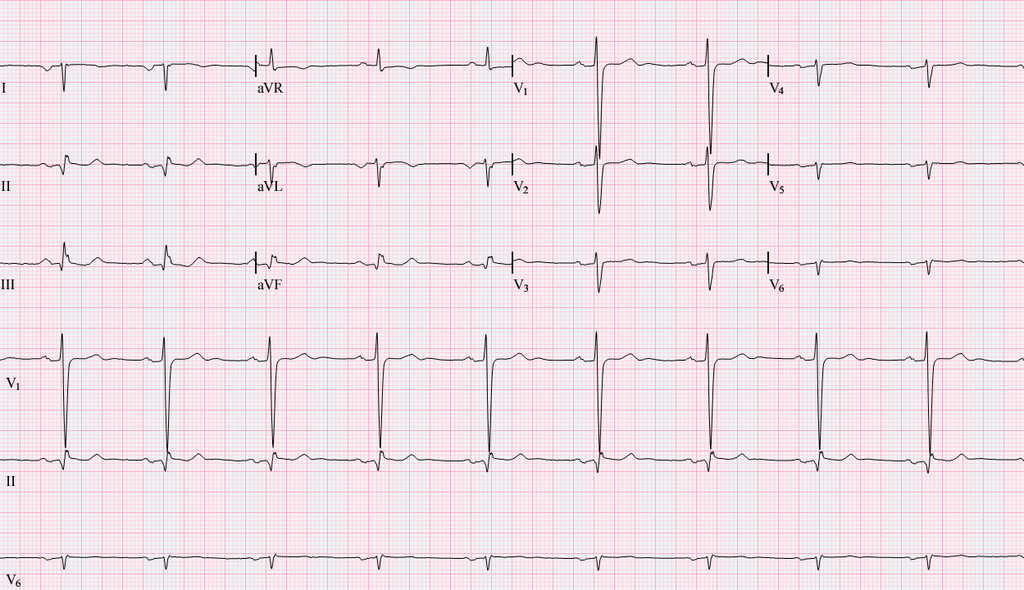
\includegraphics[width=0.7\textwidth]{./Images/img_introduccion/electrocardiograma.png}
	\caption{Electrocardiogramas}
	\label{fig:electrocardiogramas}
\end{figure}

En este proyecto se tratara de solucionar las arritmias en las que se produce una contraccion prematura del corazon
como las contracciones prematuras del corazón. Estas arritmias se 
pueden detectar con un electrocardiograma (ECG) que es un diagrama de los latidos del corazon.



\section{Algoritmo de deteccion}
Dado que para detectar arritmias correctamente se necesitan varios años de cardiologia,el algoritmo de 
deteccion que se utilizara consistira en detectar las arritmias unicamente usando los picos QRS del electrocardiograma.

Un pico QRS como se muestra en la \Cref{fig:complejoQRS} en un electrocardiograma es causado por la contaccion del ventriculo al bombear la sangre por las arterias.
Este es el impulso electrico mas fuerte que el corazon produce en cada latido. En este proyecto utilizaremos estos picos
para comparar la distancia entre ellos y poder ver si se ha producido una arritmia. 

\begin{figure}[h]
	\centering
	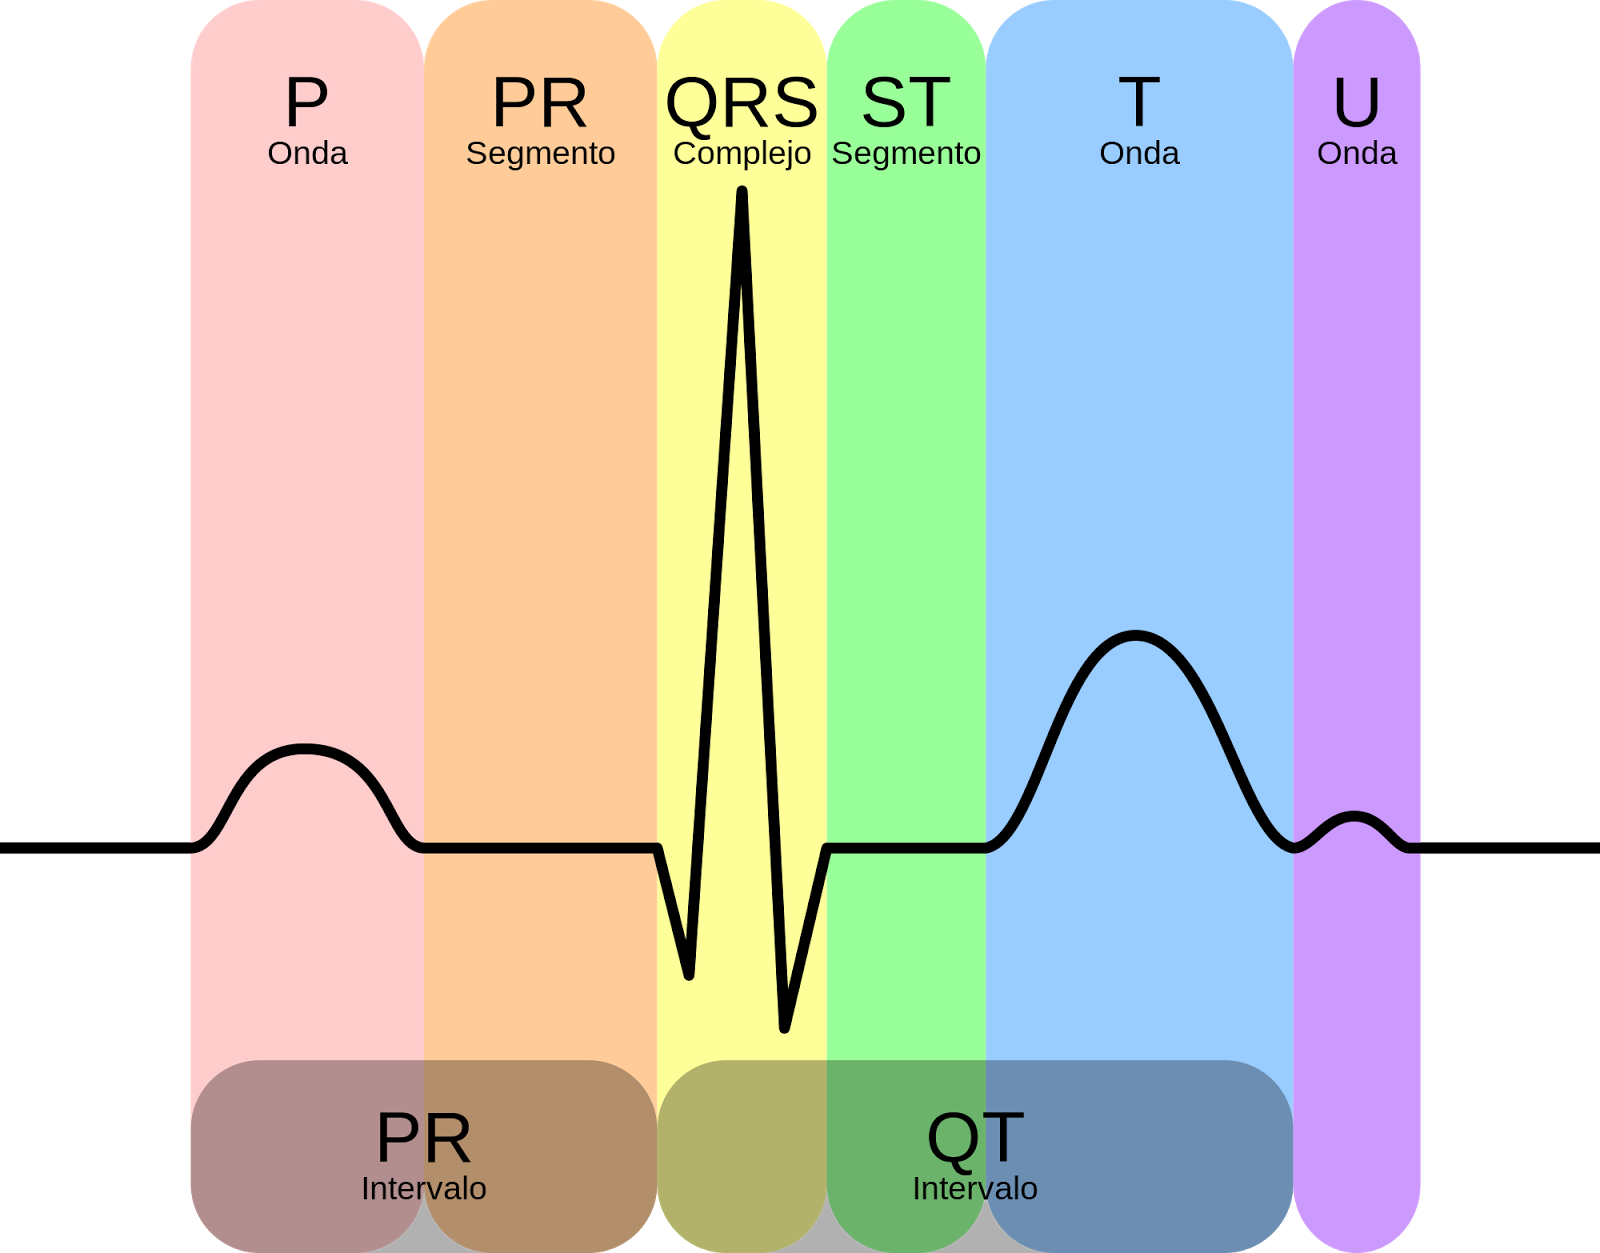
\includegraphics[width=0.4\textwidth]{./Images/img_introduccion/complejoQRS.png}
	\caption{Complejo QRS}
	\label{fig:complejoQRS}
\end{figure}

\subsection{Filtrado}
Como se puede ver en las imagenes es conveniente hacer un filtrado de las tiras de ritmo para poder detectar mejor
los picos QRS. Ya que el filtrado centra la onda en el 0 y evita fallos en el algoritmo de deteccion de picos del 
que se hablará mas adelante. 

En la creacion del proyecto se ha intentado no filtrar la onda para comprobar si se obtienen mejores resultados que
sin dicho filtrado pero no se ha dado el caso por las irregularidades de la misma.

\begin{figure}[h!]
	\centering
	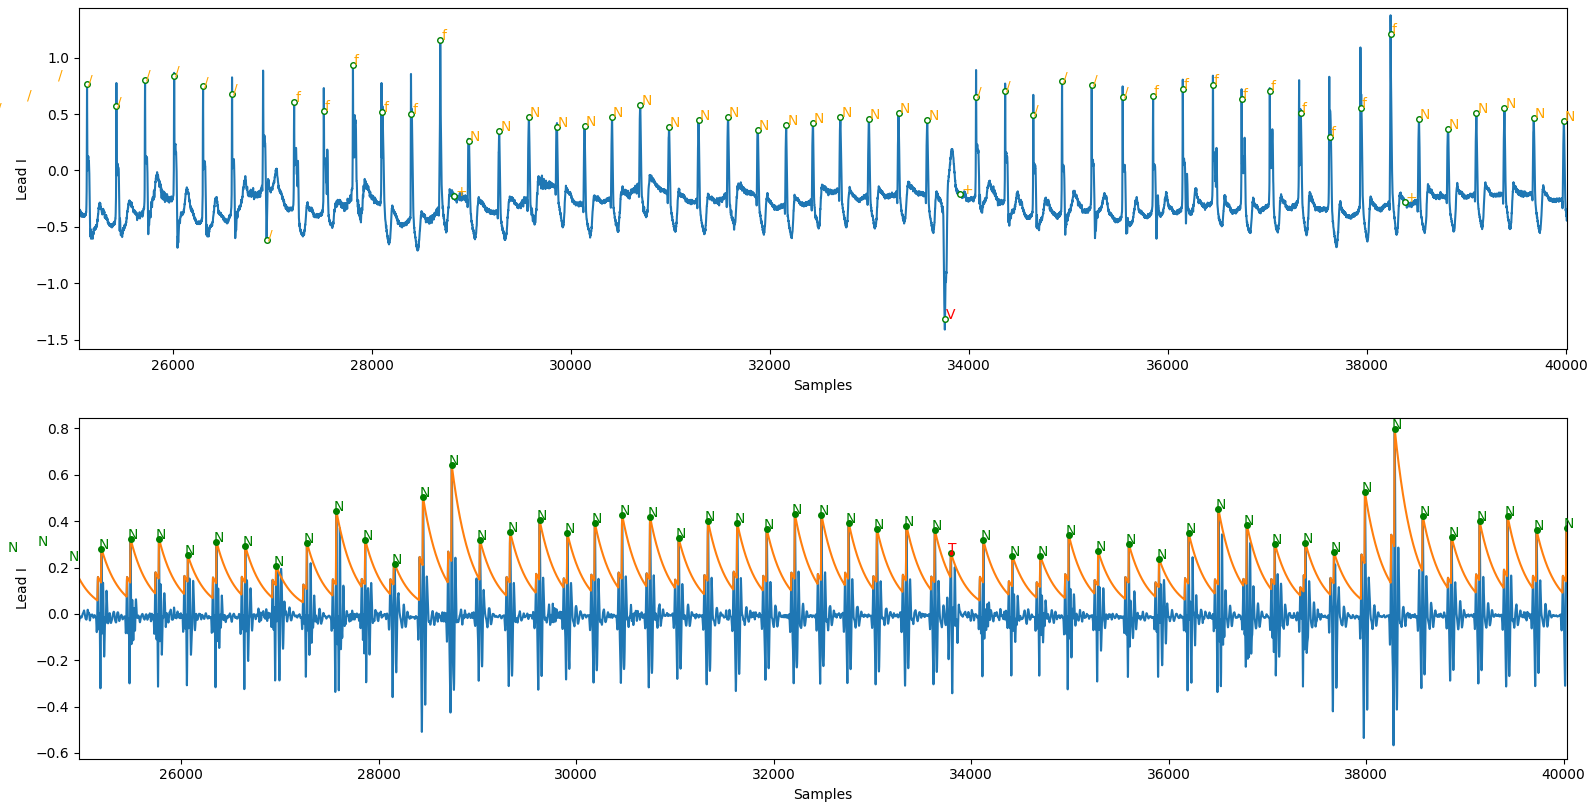
\includegraphics[width=0.99\textwidth]{./Images/img_introduccion/102filtrado_y_sin_filtrar.png}
	\caption{Ejemplo de electrocardiograma original y filtrado de paciente 102}
	\label{fig:102filtradoysinfiltrar}
\end{figure}

\section{Pruebas con pacientes}
Se han realizado las pruebas con unos resultados del Instituto de Tecnología de Massachusetts (MIT) en el que se han
recogido tiras de ritmo de media hora de varios pacientes con edades diversas y algunos de ellos llevan un marcapasos
que actua cuando el corazón no bombea la sangre lo suficientemente fuerte, es decir que el pico QRS no es tan prominente
y se necesita la ayuda de dicho marcapasos para proporcionar el impulso electrico necesario.

Estas pruebas han sido analizadas por cardiologos y se ha indicado donde el paciente padece una arritmia y donde el ritmo
es normal y donde se ha producido un error en la lectura de la señal. Tambien muestra informacion menos relevante como la 
activacion del marcapasos.

\begin{figure}[h]
	\centering
	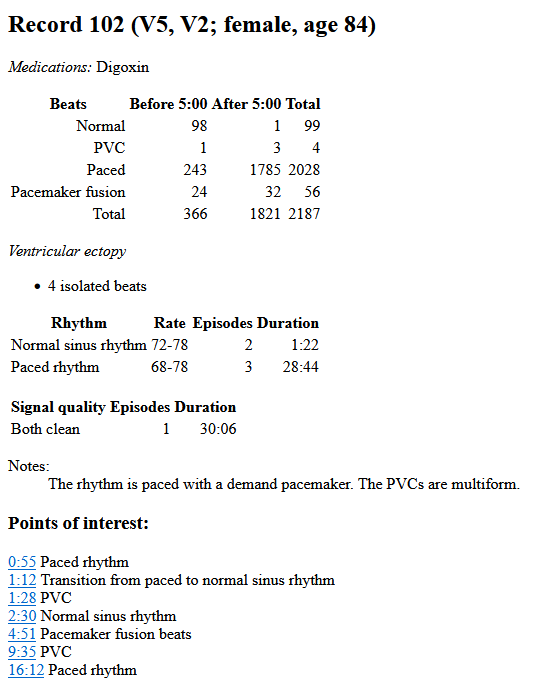
\includegraphics[width=0.6\textwidth]{./Images/img_introduccion/Paciente_pruebas_MIT.png}
	\caption{Ejemplo con paciente 102}
	\label{fig:Paciente_pruebas_MIT}
\end{figure}

\section{Utilizacion de las FPGAs}
Este proyecto requiere un gran procesamiento de señales, una alta cantidad de calculos y un eficiente paralelismo 
entre modulos por ello la mejor forma de optimizar el algoritmo es utilizando una FPGA.

Los motivos son los siguientes:

\begin{itemize}
	\item Las FPGA pueden procesar datos a velocidades muy altas, lo que lo hace indispensable para esta aplicacion
	 que esta pensada para ejecutarse en tiempo real.
	\item Las FPGA son dispositivos de hardware programable que permite diseñar circuitos digitales personalizados, 
	y por ello pueden reconfigurarse para adaptarse a tareas específicas. Ademas son susceptibles a cambios en el 
	algoritmo para una posible mejora de este.
	\item El alto paralelismo que ofrecen las FPGA es perfecto para las multitareas que realiza el algoritmo.
	\item Puesto que las FPGA pueden ser diseñadas para realizar una tarea en concreto, estas son mas energeticamente
	eficientes que otros dispositivos como los portatiles.
\end{itemize}

Para este proyecto se usara la FPGA Basys3 de Artix-7 para probar el funcionamiento del algoritmo. Aunque se debe considerar, segun
la cantidad de datos introducidos, que en este caso seria la longitud de la señal segun el tiempo transcurrido, utilizar
una FPGA cuyo hardware pueda soportar dicha cantidad de datos.


\section{Objetivos del proyecto y organización}
Los objetivos de este proyecto es tener una solucion para detectar contracciones prematuras ventriculares a tiempo real en
un largo periodo de tiempo y optimizar el algoritmo para que se ejecute de una forma mas eficiente y menos costosa en una FPGA

Para ello la organizacion de este proyecto comienza con la creacion de el prototipado del algoritmo en software para facilitar
la manera de probar el algoritmo con la solucion proporcionada por la base de datos y poder ver resultados graficos, para mejorar
la velocidad de compilacion y depuracion del algoritmo, para aumentar la claridad del algoritmo que se quiere conseguir en el
prototipado y para validar la funcionalidad y eficacia del algoritmo.
\section{Analisis y optimizacion del algoritmo}
Para lograr los objetivos del algoritmo se centra en tres funciones.
\begin{enumerate}
	\item Filtrado de la señal original: Lo que hace que la señal sea mas facil de procesar para encontrar los picos QRS.
	 Esto se realiza multiplicando los valores de la señal original por los valores de filtrado.
	\item Deteccion de picos sobre la señal filtrada: Se analiza cada señal y comparandola con otras señales anteriores se
	 deduce si puede ser un posible pico y si lo es, se comprueba si es un pico QRS.
	\item Deteccion de arritmias comparando la posicion de los picos: una vez se tienen los picos QRS se calcula la distancia
	 de el pico actual con el pico anterior y dependiendo de las otras distancias se calcula si hay una arritmia.
\end{enumerate}


\section{Implementacion en la FPGA}
Para implementar el codigo en la FPGA se implementaran varios modulos para tratar de imitar el proyecto creado en software 
los modulos mas importantes son.

	\begin{enumerate}
		\item Modulo de filtrado: Se guardan los valores del filtrado en una memoria y se van multiplicando los valores que van llegando 
		al modulo. estos valores multiplicados a su vez se almacenan en memoria hasta que pasan al siguente módulo
		\item Deteccion de picos sobre la señal filtrada: Se analiza cada señal que pasa del modulo de filtrado y mediante una maquina de estados
		se busca el pico mas alto dentro de los limites del cutoff, si se encuentra se comprueba si es un pico QRS.
		\item Deteccion de arritmias comparando la posicion de los picos: una vez se tienen los picos QRS se implementa una maquina de estados que
		sea capaz de hallar la distancia entre 2 picos, meterla en un buffer y calcular el porcentaje de el tamaño de la distancia con las demas.
	\end{enumerate}

	Estos modulos tratan de replicar las funcionalidades que realiza el algoritmo de software y se convertiran en la parte esencial
	de dicho programa. 
	
	Además de estos modulos se debe de crear un modulo que acompase a estos tres y un testbench para probar el funcionamiento
	del programa en la simulación.
	\chapter{Planteamiento del algoritmo en software}
\section{Recopilacion de los datos}
Para la recopilacion de los datos se utilizara la libreria wfdb que se encarga de proporcionar
funciones para leer y escribir archivos de diferentes formatos que contienen señales biomédicas,
como archivos de registro de señales (por ejemplo, formato .dat), archivos de anotaciones
 (por ejemplo, formato .atr) y archivos de cabecera (por ejemplo, formato .hea).

 Los pacientes vienen identificados por un id (por ejemplo, 101) y hay 3 ficheros por paciente, 
 con extensiones .dat, .atr y .hea

Se descarga la base de datos con la funcion de la libreria de wfdb, dldatabase que recoge 
la señal del paciente y las anotaciones de los cardiologos sobre cada pico QRS.


\lstset{language=python, breaklines=true, basicstyle=\footnotesize}
\begin{lstlisting}[frame=single]
#download the database if not available
if os.path.isdir("mitdb"):
	print('You already have the data.')
else:
	wfdb.dl_database('mitdb', 'mitdb')
\end{lstlisting}

Los pacientes de la base de datos se han hecho una prueba de 30 mins lo que en la señal 
equivale a 650000 samples.

\lstset{language=python, breaklines=true, basicstyle=\footnotesize}
\begin{lstlisting}[frame=single]
sampfrom = 0
sampto = 650000
record = wfdb.rdsamp('mitdb/102', sampfrom=sampfrom, sampto=sampto)
annotation = wfdb.rdann('mitdb/102', 'atr', sampfrom=sampfrom, sampto=sampto)
\end{lstlisting}

Por ultimo, para visualizar esta señal con las anotaciones de los cardiologos y poder comparar 
con las anotaciones que realiza el algoritmo se usara la libreria matplotlib.pyplot.

Con esto se mostrara la señal original con las anotaciones y la señal filtrada con las anotaciones
del algoritmo como en \Cref{fig:102filtradoysinfiltrar}

\lstset{language=python, breaklines=true, basicstyle=\footnotesize}
\begin{lstlisting}[frame=single]
#plot the signal
#add markers to the original signal
ax[0].plot(original_signal)
ax[1].plot(filtered_signal)
ax[0].set_xlabel('Samples')
ax[0].set_ylabel('Lead I')
ax[1].set_xlabel('Samples')
ax[1].set_ylabel('Lead I')


#Making the upper signal
for pos, sym in zip(annotation.sample, annotation.symbol):
    pos -= sampfrom
    ax[0].plot(pos, original_signal[pos], 'go', markersize=4, markerfacecolor='white')
    if(sym == "A" or sym == "V" or sym == "a"):
        ax[0].text(pos+10, original_signal[pos], sym, color='red')
    else:
        ax[0].text(pos+10, original_signal[pos], sym, color='orange')
\end{lstlisting}

\section{Filtrado de la señal original}
Este filtrado es llevado a cabo por el filtrado IIR.

El filtrado IIR, que significa "Infinite Impulse Response" (respuesta infinita al impulso),
es un tipo de filtro utilizado en el procesamiento de señales digitales y analógicas.

La formula que se utilizara para el filtrado es

\[ Y[i] = \sum_{k=0}^{N_x -1} b_k \cdot x[i-k] \]

Con lo que b son los coeficientes y x la señal a filtrar

Los coeficientes se trata de un buffer de 99 valores en punto flotante simetricos que se iteran de forma 
circular, con lo que despues de ejecutar el ultimo valor vuelve de nuevo al primero.  

Para el filtrado se usa la funcion lfilter de la libreria scipy.signal

\lstset{language=python, breaklines=true, basicstyle=\footnotesize}
\begin{lstlisting}[frame=single]
    filtered_signal = lfilter(filter_taps_99_6_28, 1.0, original_signal)
\end{lstlisting}
TODO a y formula completa ademas de una mejor explicacion

\section{Detección de picos QRS}

El algoritmo de deteccion de picos esta representada en esta funcion que 
recibe la señal filtrada e intenta detectar los picos QRS.

Este algoritmo esta basado en el que se usa en el documento  https://www.mdpi.com/2079-9292/10/19/2324 
donde en el 4.1.2 muestran una maquina de estados del proceso que realizan.

\begin{figure}[h!]
    \centering
    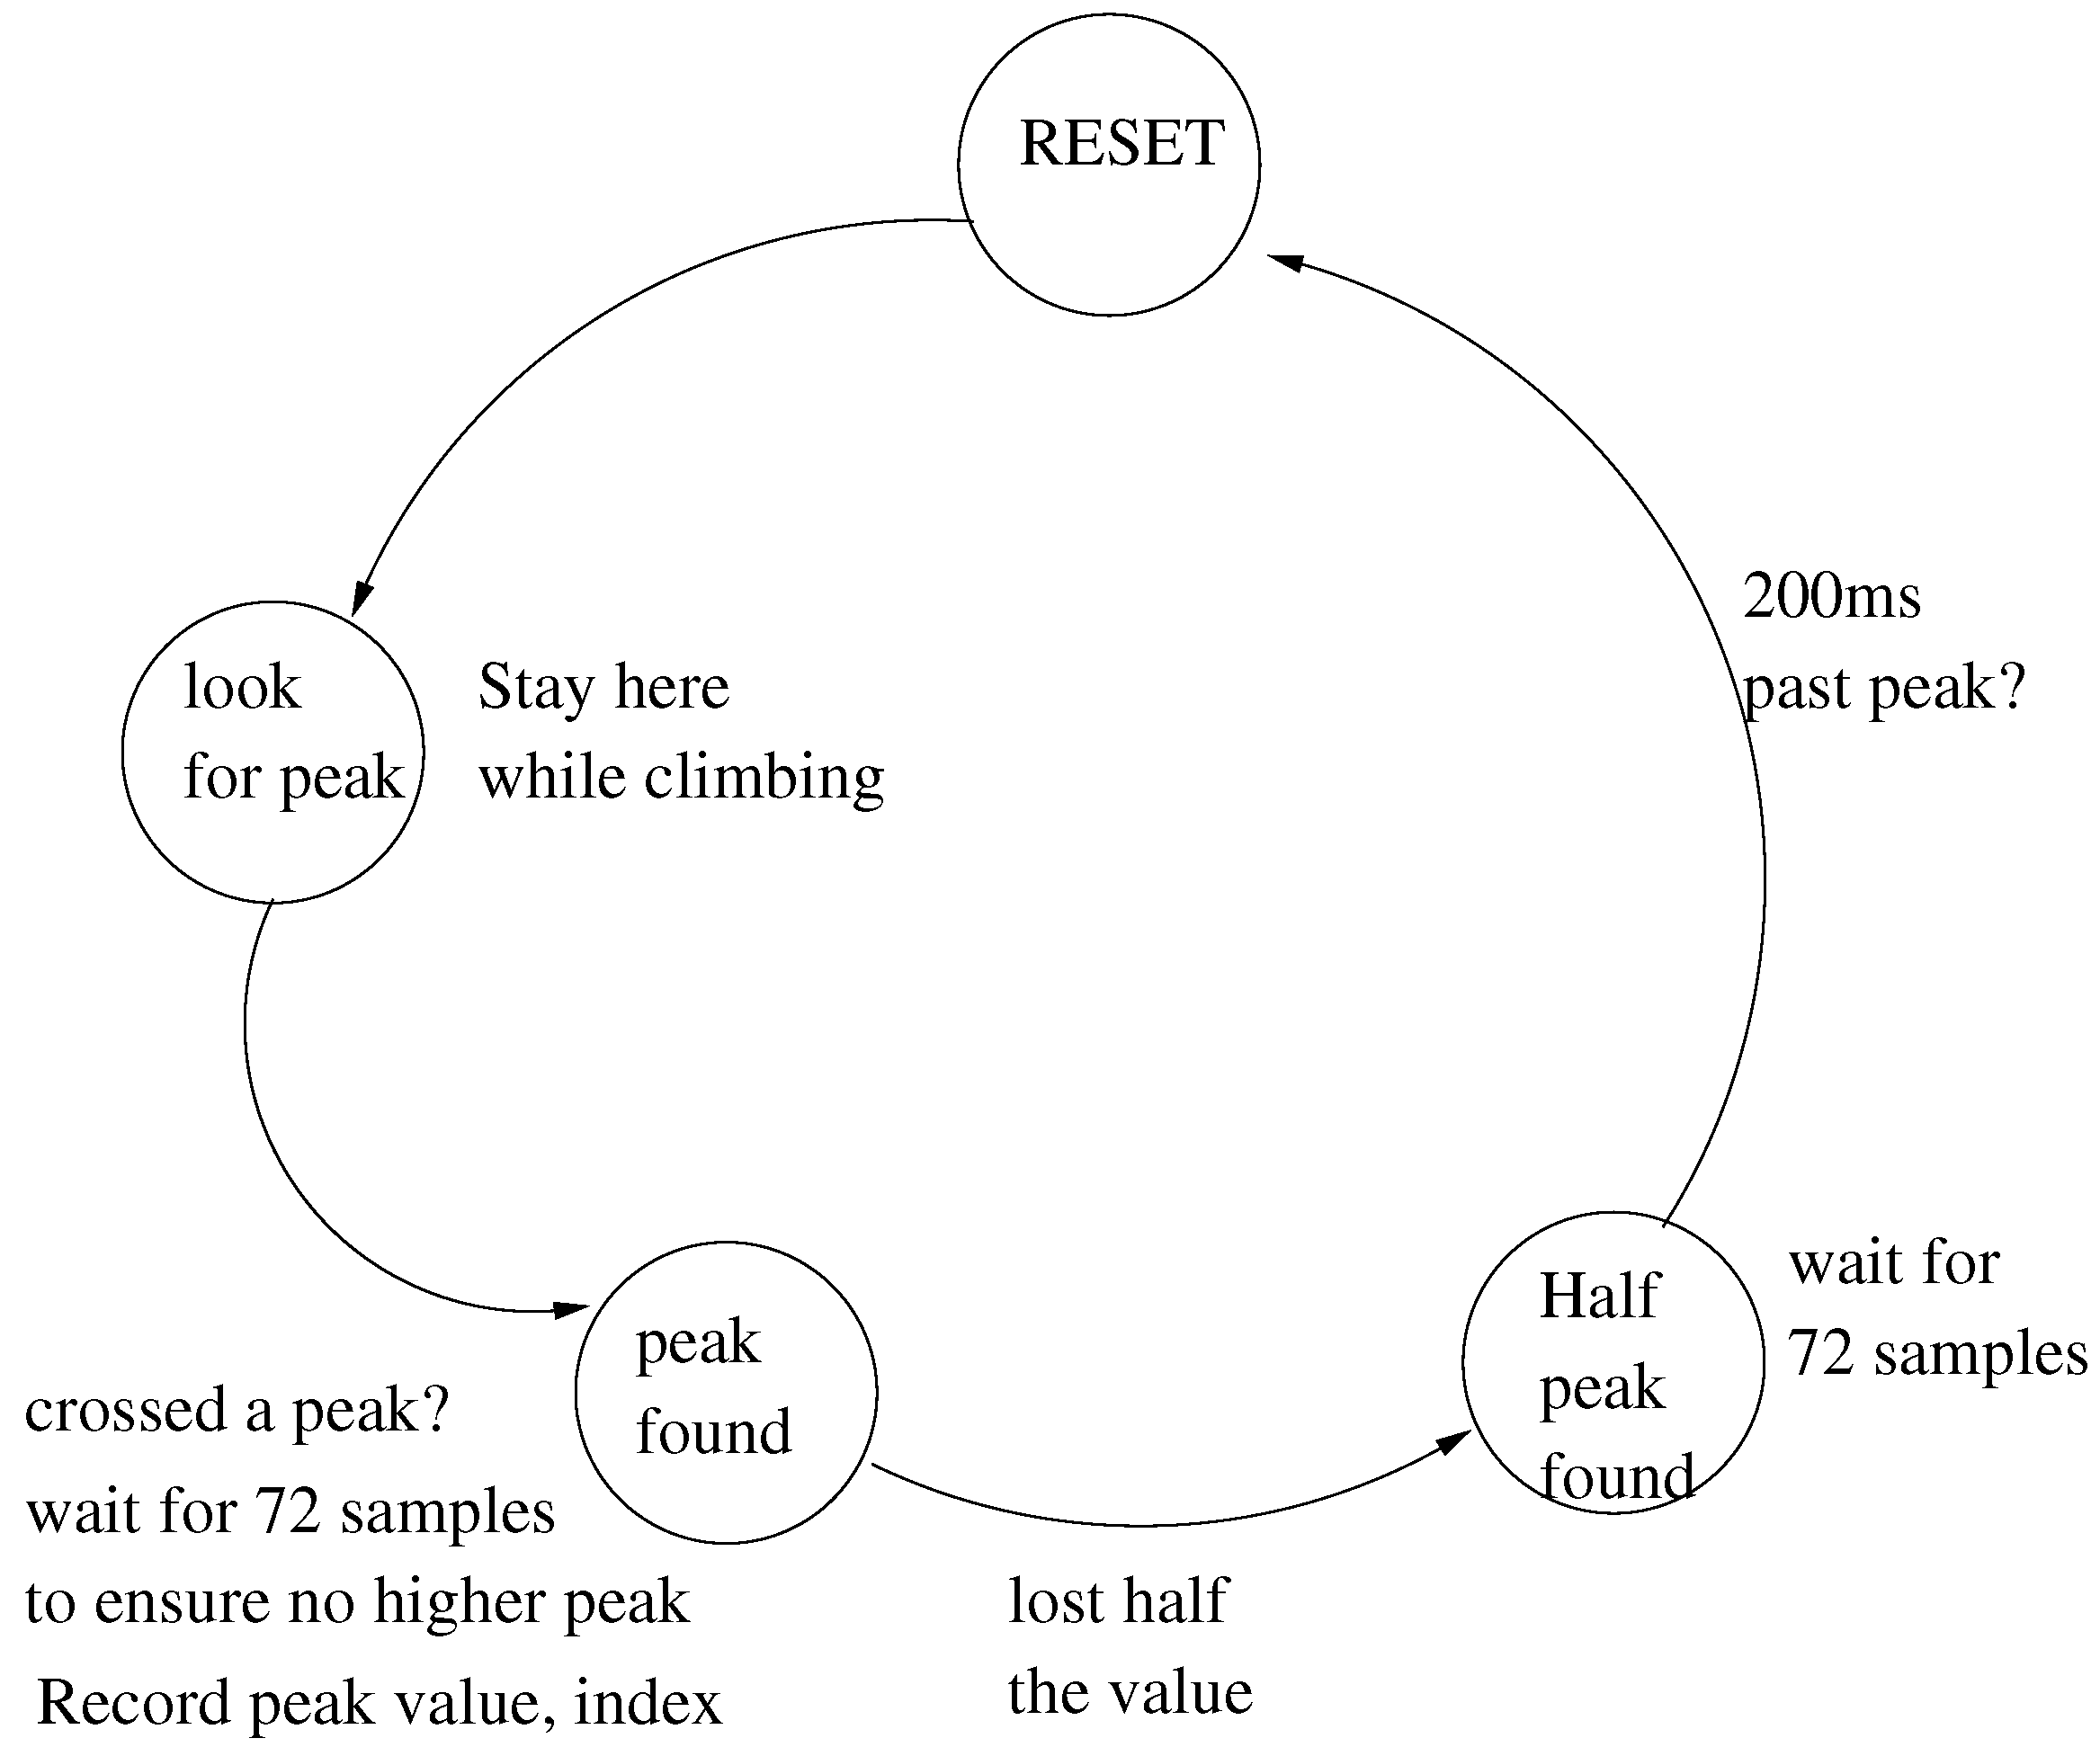
\includegraphics[width=0.6\textwidth]{./Images/img_algoritmo/fsm_mdpi.png}
    \caption{Maquina de estados de algoritmo de deteccion de picos de estudio de caracterizacion de señales usando polinomios de Hermite}
    \label{fig:fsm_mpdi}
\end{figure}

Si bien nuestro algoritmo es distinto a ese, se replica el esperar a 72 muestras
para asegurar de que no se encuentra un pico superior y asi considerarlo como un pico QRS.

Es por ello que definimos la variable \lstinline|samples_around_peak| como 72 para comparar dicha condición.

Para hallar el pico mas alto se necestia definir un pico en last\_peak y si se encuentra otro pico se produce

\lstset{language=python, breaklines=true, basicstyle=\footnotesize}
\begin{lstlisting}[frame=single]
last-peak = max(last-peak,signal[i])
\end{lstlisting}

Sin embargo hay un problema y es que cuando se detecte un pico QRS, es decir cuando se haya detectado el pico 
mas alto despues de haber pasado 72 samples se restauran los valores para empezar a detectar nuevos picos y al
haber ruido el algoritmo podria detectar falsos picos QRS asi que por ello se implementa un cutoff.

El cutoff es representado como una funcion descendente que parte de cada pico localizado y mientras no se haya
encontrado ningun pico, el valor de dicha funcion va decreciendo. La principal funcion del cutoff es evitar que
el algoritmo detecte picos con el ruido y por ello se ha ajustado para que no ocurra el problema anterior y 
ser capaz de detectar todos los picos QRS.

La funcion del cutoff es la siguiente.
\lstset{language=python, breaklines=true, basicstyle=\footnotesize}
\begin{lstlisting}[frame=single]
def calcular_cutoff(cutoff):
    cutoff = cutoff - cutoff/(256 - 64)
    return cutoff
\end{lstlisting}

Esta funcion es llamada cuando no se ha encontrado un nuevo pico y decrementa su valor, cuando se localiza un
nuevo pico, el cutoff pasa a tener el valor del pico localizado.

Se han dado los valores (256 - 64) a la formula para que fuese mas facil la divison en hardware pero como al final 
se acabo haciendo en un modulo de division en punto flotante cualquier valor es valido para la division aunque debido 
al buen desempeño del valor en el programa se decidio dejar asi.

\lstset{language=python, breaklines=true, basicstyle=\footnotesize}
\begin{lstlisting}[frame=single]
    def extract_peak_indices(signal, total_samples):
        samples_around_peak = total_samples // 2
        last_peak = None
        last_index = None
        peak_indices = []
        cutoff = 0
        for i in range(samples_around_peak-1, len(signal)):
            if last_peak == None:
                last_peak = signal[i]
                last_index = i
                cutoff = calcular_cutoff(cutoff)
            else:
                if signal[i] > last_peak and signal[i] > cutoff:
                    last_peak = signal[i]
                    last_index = i
                    cutoff= signal[i]
                else:
                    if (i - last_index) >= samples_around_peak and last_peak > cutoff:
                        peak_indices.append(last_index)
                        cutoff = calcular_cutoff(cutoff)
                        last_peak = None
                        last_index = None         
                    else:
                        cutoff = calcular_cutoff(cutoff)
            cutoff_plot.append(cutoff)
        ax[1].plot(range(samples_around_peak-1, len(signal)),cutoff_plot)
        return peak_indices
\end{lstlisting}

La salida de dicha funcion es un buffer de samples que sirven como indices para indicar donde se han encontrado
los picos QRS y asi poder pasar al modulo de deteccion de arritmias.

\section{Detección de arritmias}

El algoritmo de deteccion de arritmias se encarga de ver si se ha producido una arritmia segun la
distancia entre los picos.

En la deteccion de arritmias es de vital importancia establecer un límite en la distancia entre los picos
para poder considerar que ha habido una arritmia o no, esta tarea solo se pudo hacer probando con diferentes
rangos y viendo el indice de aciertos producidos en las pruebas a cada paciente de las que se hablara más adelante. 

El algoritmo va almacenando distancias entre los picos QRS (es por ello que en la primera iteración no se almacena nada)
y se declaran varias variables.

\begin{itemize}
    \item last\_distance: se utiliza para almacenar la ultima distancia recogida y asi poder compararla con la distancia 
    actual en calculos posteriores
    \item counter\_buffer: utilizado para tener el valor de la posicion del buffer donde se escribe.
    \item counter\_arrythmia: utilizado para indicar si la distancia anterior fue una arritmia.
    \item TNRange: Se utiliza para indicar si hay una distancia mas grande de lo normal entre 2 picos QRS producido
    por una arritmia. Es importante tener esta distancia en cuenta ya que si el ritmo del paciente vuelve a la
    normalidad se compararia la distancia entre el ritmo normal del paciente con el ritmo extendido por la arritmia,
    ya que de no tenerlo en cuenta el algoritmo lo clasificaria como arritmia como se puede ver en la \cref{fig:senial_explicacion_TNRANGE}, por ello se compara con un valor anterior
    que sea el ritmo normal del paciente.
\end{itemize}

\begin{figure}[h!]
    \centering
    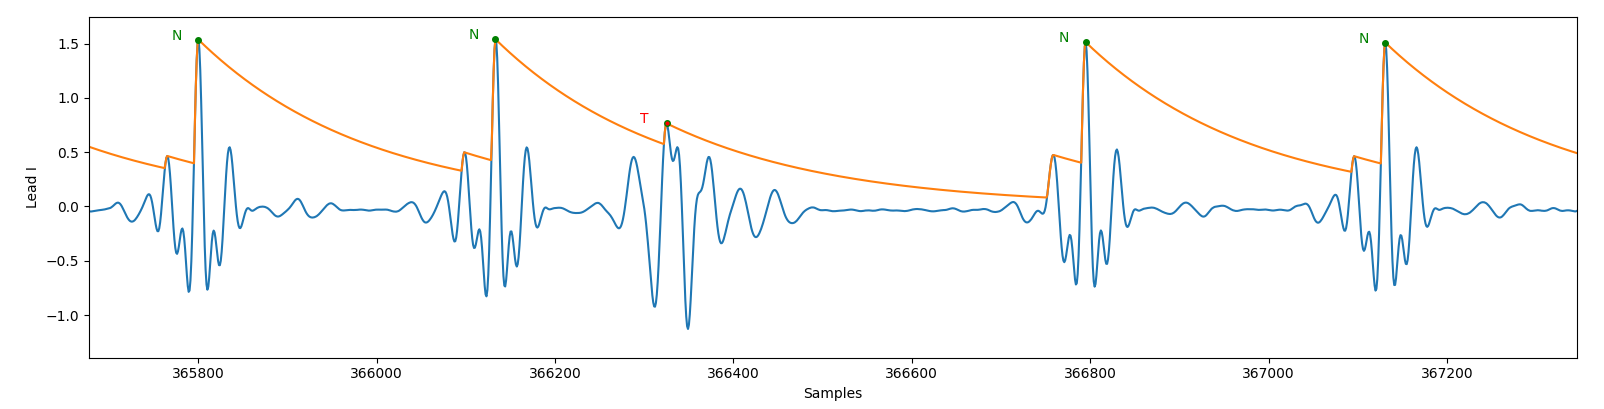
\includegraphics[width=0.9\textwidth]{./Images/img_algoritmo/senial_explicacion_TNRANGE.png}
    \caption{Cuando se detecta una arritmia, a veces, la siguiente distancia es considerablemente mas grande de lo normal. Para no detectar falsos positivos, se omite esa distancia}
    \label{fig:senial_explicacion_TNRANGE}
\end{figure}

Por ello si se ha detectado una arritmia, la siguiente distancia se compara con
la tercera ultima distancia escrita en el buffer que posiblemente sea una distancia causada por un ritmo normal. 
Si no se da el caso, se compara con last\_distance.

la funcion que compara las distancias devuelve un char que va a ser el que se vaya a plotear en la grafica, 
si el char es "N" significa que se ha detectado un ritmo normal y por tanto solo se plotea. Sin embargo si el 
resultado es "T" significa que la distancia es mas corta de lo normal, se detecta la arritmia y se ponen
counter\_arritmia a 1 para saber que la distancia es mas corta y TNRange a true para que el algoritmo sepa 
que la distancia que venga despues puede ser una ampliada. 

\lstset{language=python, breaklines=true, basicstyle=\footnotesize}
\begin{lstlisting}[frame=single]
    #init the first distance, the first beat doesn't count
    posant = peaks[0]
    last_distance = peaks[1] - peaks[0]

    pos_buffer = [last_distance]
    counterBuffer = 0
    #this var refers to the distance left in between an arrythmia and normal rythm 
    # which tends to be longer. To avoid detection problems we will not compare this distance so the detection can be more precise
    TNRange = False
    counter_arrrythmia = 0
    for pos in peaks[1:]:
        act_distance = pos - posant
        pos_buffer.append(act_distance)
        counterBuffer += 1
    
        if(TNRange==True and counter_arrrythmia == 0):
            sym = get_frecuency_in_char(pos_buffer[counterBuffer - 3],act_distance)
    
            TNRange=False
        else:
            if(TNRange == True):
                counter_arrrythmia -= 1
            sym = get_frecuency_in_char(last_distance,act_distance)
        
    
        if(sym == "N"):
            ax[1].plot(pos, filtered_signal[pos], 'go', markersize=4, markerfacecolor='green')
            ax[1].text(pos-30, filtered_signal[pos], sym, color='green')       
        elif(sym == "T"):
            ax[1].plot(pos, filtered_signal[pos], 'go', markersize=4, markerfacecolor='red')
            ax[1].text(pos-30, filtered_signal[pos], sym, color='red')
            TNRange = True
            counter_arrrythmia = 1
        
        posant = pos
        last_distance = act_distance
\end{lstlisting}

La funcion get\_frecuency\_in\_char() se encarga de calcular las distancias entre el ritmo actual y un ritmo normal. 
Para ello recibe como entrada ambas distancias.

Para empezar se calcula el gap que es simplemente la diferencia que tiene el la distancia anterior con la actual.
Despues se calcula el porcentaje de la diferencia de distancia con la distancia anterior que sabemos que va a ser 
un ritmo normal.

Si ese porcentaje es mayor que el 15\% entonces se considera que la distancia normal es mucho mayor que la actual
y por tanto como la distancia actual entre 2 picos es pequeña, se da por hecho que hay una arrimtia.

Notese que no le damos importancia si el gap da como resultado un número negativo de cualquier tamaño, esto se debe
a que este proyecto solo esta pensado para detectar contracciones prematuras del corazon, por ende solo necesitamos 
saber si la distancia actual es menor que la anterior. Además ningun paciente parece padecer ninguna arritmia de otro
tipo.

\lstset{language=python, breaklines=true, basicstyle=\footnotesize}
\begin{lstlisting}[frame=single]
def get_frecuency_in_char(last_distance,act_distance): 

    gap = last_distance - act_distance

    percentaje = (gap / last_distance) * 100

    if(percentaje > 15):
        ret = "T"
    else:
        ret = "N"
    return ret

\end{lstlisting}

\section{Pruebas con el algoritmo}

Se han realizado una serie de pruebas para probar el algoritmo estas se encargan de comprobar si las posiciones donde
se ha detectado un pico QRS coinciden con las posiciones de los picos detectados por los cardiologos, y ademas se 
encargan de comparar las anotaciones de los cardiologos con las generadas por el algoritmo.

Con estas estadisticas es posible comparar el porcentaje de aciertos, en los que se comprende el numero de 
falsos positivos, (referido a los ritmos normales que el algoritmo considara arritmias) y 
falsos negativos (referido a las arrimtias que el algoritmo considera un ritmo normal).

Para desarrollar estas pruebas, se crea una clase Pair que contenga por cada iteracion de la deteccion de arritmias, el simbolo sacado 
por el algoritmo y la posicion del sample en la que se encuentre dicho pico QRS.

\lstset{language=python, breaklines=true, basicstyle=\footnotesize}
\begin{lstlisting}[frame=single]
class Pair:
def __init__(self, sym, pos):
    self.sym = sym
    self.pos = pos

def __repr__(self):
    return f"Pair({self.sym}, {self.pos})"

\end{lstlisting}

Dicho objeto se inserta en un buffer para luego poder comparar con las anotaciones de la señal original.

\lstset{language=python, breaklines=true, basicstyle=\footnotesize}
\begin{lstlisting}[frame=single]
if(sym == "N" or sym == "T"):
    pair = Pair(sym,pos)    
    produced_symbols.append(pair)
\end{lstlisting}

Una vez se rellena todo el buffer de Pares, se comprueban 2 cosas.
\begin{enumerate}
	\item Si se ha detectado un pico QRS en la señal filtrada y se
     corresponde con el pico de la señal original situado en un sample de una posicion aproximada.
	\item Si,en el caso de que se haya detectado el pico, las anotaciones de los cardiologos coinciden
     con las generadas por el algoritmo
\end{enumerate} 

Para este proyecto, solo se valora si el paciente tiene un ritmo normal o una arritmia, pero las anotaciones
que contiene la señal original pueden simbolizar otros problemas como la entrada del marcapasos o otros problemas con la onda T.
En la clase Annotation de la libreria wfdb, vienen explicadas todas las posibles anotaciones que puede haber.
\lstset{language=python, breaklines=true, basicstyle=\footnotesize}
\begin{lstlisting}[frame=single]
    ann_labels = [
        AnnotationLabel(0, " ", 'NOTANN', 'Not an actual annotation'),
        AnnotationLabel(1, "N", 'NORMAL', 'Normal beat'),
        AnnotationLabel(2, "L", 'LBBB', 'Left bundle branch block beat'),
        AnnotationLabel(3, "R", 'RBBB', 'Right bundle branch block beat'),
        AnnotationLabel(4, "a", 'ABERR', 'Aberrated atrial premature beat'),
        AnnotationLabel(5, "V", 'PVC', 'Premature ventricular contraction'),
        AnnotationLabel(6, "F", 'FUSION', 'Fusion of ventricular and normal beat'),
        AnnotationLabel(7, "J", 'NPC', 'Nodal (junctional) premature beat'),
        AnnotationLabel(8, "A", 'APC', 'Atrial premature contraction'),
        ...
        AnnotationLabel(12, "/", 'PACE', 'Paced beat'),
        AnnotationLabel(13, "Q", 'UNKNOWN', 'Unclassifiable beat'),
        AnnotationLabel(14, "~", 'NOISE', 'Signal quality change'),
        AnnotationLabel(16, "|", 'ARFCT',  'Isolated QRS-like artifact'),
        ...
        AnnotationLabel(38, "f", 'PFUS',  'Fusion of paced and normal beat'),
        ...
    ]
\end{lstlisting}

Por ello en este proyecto solo se prestara atencion a la anotacion A y a la anotacion V que simbolizan 
las contacciones prematuras de la auricula y el ventriculo, las demas anotaciones sobre el pico QRS seran 
consideradas como ritmos normales.

Para poder ver donde se pueden producir posibles errores y el tipo de estos se ha creado un buffer donde en 
cada iteracion se hace push de un string con el resultado de la señal filtrada y la señal original.

Si por otro lado, el pico no se ha detectado donde tendria que haber un pico QRS puesto en la señal original, 
se pone \"--\" para simbolizarlo.

Como se menciono anteriormente la deteccion de picos sobre a señal filtrada es aproximado, por lo que se cuenta
si se ha detectado un pico 50 samples antes del pico de la señal original y 50 picos despues. El numero de aproximacion 
es moderadamente mas amplio para evitar problemas con las posibles imprecisiones del filtrado.  

Otra prueba que se realiza es un conteo de las anotaciones correctas en total, las anotaciones incorrectas en total, las anotaciones
correctas solo de los picos detectados como arritmia, las incorrectas de ese mismo tipo, y los picos no registados. 

\lstset{language=python, breaklines=true, basicstyle=\footnotesize}
\begin{lstlisting}[frame=single]
def test_arrythmias(original_symbols,produced_symbols):
    sol = []
    #stats parameters
    detected = 0
    undetected = 0
    correctValue = 0
    incorrectValue = 0
    correctArrythmia = 0
    incorrectArrythmia = 0
    
    for i in range(len(original_symbols)):
        found = False
        aproximation = 5
        for j in range(len(produced_symbols)):
            if((produced_symbols[j].pos - 50) > original_symbols[i].pos - aproximation and (produced_symbols[j].pos - 50) < original_symbols[i].pos + aproximation):
                found = True
                sol.append(""+produced_symbols[j].sym + original_symbols[i].sym)
                detected += 1
                
                if produced_symbols[j].sym == 'N' and (original_symbols[i].sym == 'N' or original_symbols[i].sym == '/' or original_symbols[i].sym == 'f' or original_symbols[i].sym == 'L'):
                    correctValue += 1
                elif produced_symbols[j].sym == 'T' and (original_symbols[i].sym == 'A' or original_symbols[i].sym == 'V' or original_symbols[i].sym == 'a'):
                    correctValue += 1
                    correctArrythmia += 1
                elif produced_symbols[j].sym == 'T' and (original_symbols[i].sym == 'N' or original_symbols[i].sym == '/' or original_symbols[i].sym == 'f'or original_symbols[i].sym == 'L'):
                    incorrectValue += 1
                    incorrectArrythmia += 1
                elif produced_symbols[j].sym == 'N' and (original_symbols[i].sym == 'A' or original_symbols[i].sym == 'V'):
                    incorrectValue += 1
                    incorrectArrythmia += 1
                else:
                    incorrectValue += 1
                
        if(found==False):
            sol.append("--")
            undetected += 1
\end{lstlisting}

Con el conteo de las anotaciones se pueden sacar varias conclusiones aparte de las dichas 
anteriormente como los picos totales que tiene la señal original, el procentaje de picos 
detectados, el porcentaje de picos no detectados, el porcentaje de arritmias detectadas 
correcetamente, el porcentaje de falsos positivos o falsos negativos, y el porcentaje de exito de deteccion de 
arritmias segun todas las arrimtias contando falsos positivos y negativos.

\begin{figure}[h!]
	\centering
    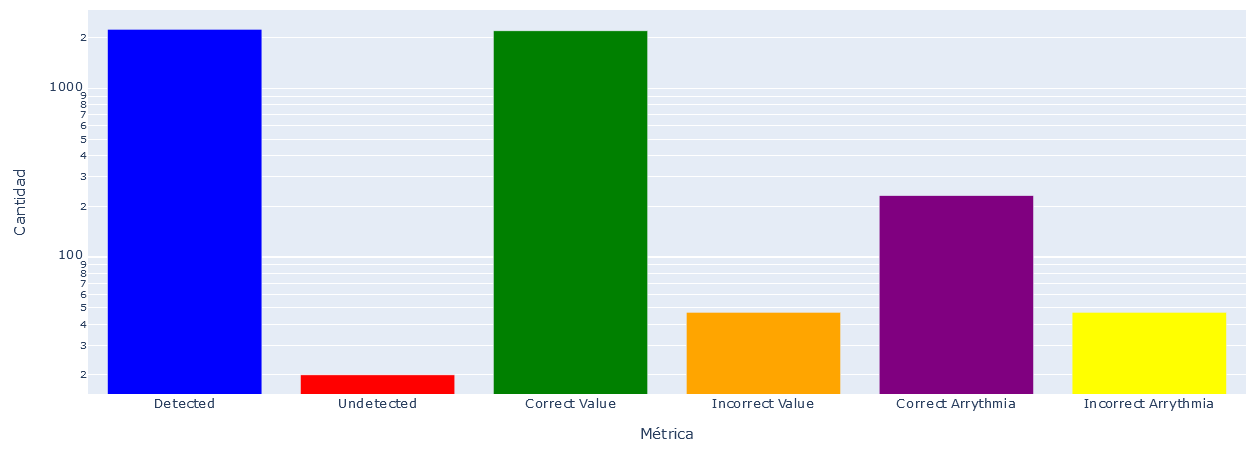
\includegraphics[width=0.99\textwidth]{./Images/img_algoritmo/estadisticas_arritmias_1.png}
    \caption{Estadisticas}
    \label{fig:estadisticas_algoritmos_1}
\end{figure} 

\begin{figure}[h!]
	\centering
    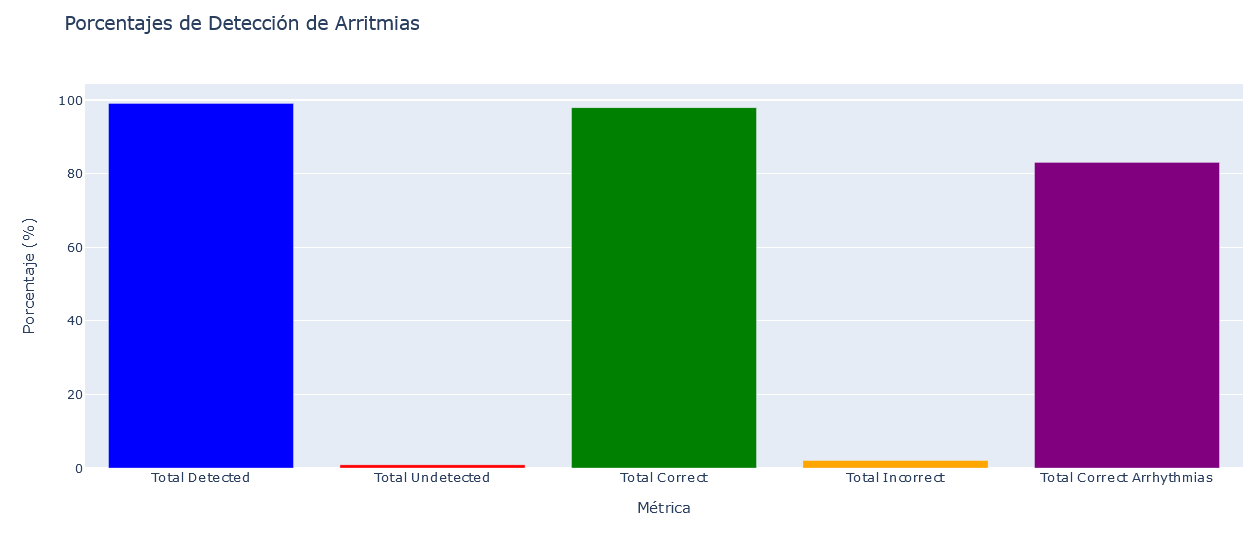
\includegraphics[width=0.99\textwidth]{./Images/img_algoritmo/estadisticas_arritmias_2.png}
    \caption{Porcentaje de las estadisticas}
    \label{fig:estadisticas_algoritmos_2}
\end{figure} 


Las pruebas que se han realizado se aplican solo para un paciente pero es posible aplicar estas pruebas a todos los pacientes.
Para ello se ha creado un nuevo fichero de python que se encarga de realizar la misma prueba para los pacientes cuyo id esta
almacenado en un buffer.

Este programa tiene 2 modos, uno procesa un paciente individualmente y el otro itera la lista definida procesandolos a todos. La
logica del algoritmo esta contenida en una nueva funcion llamada calculations().

\lstset{language=python, breaklines=true, basicstyle=\footnotesize}
\begin{lstlisting}[frame=single]
    mode = input("Introduce 1 to process only a patient or 2 to process all (monster mode): ")
if mode == "1":
    patientNumber = input("introduce the patient number: ")
    #select the data quantity (650000 sample intervals)
    sampfrom = 0
    sampto = 650000
    record = wfdb.rdsamp("mitdb/"+patientNumber, sampfrom=sampfrom, sampto=sampto)
    annotation = wfdb.rdann("mitdb/"+patientNumber, 'atr', sampfrom=sampfrom, sampto=sampto)
    calculations(sampfrom,sampto,record,annotation)
    perc = test_arrythmias(original_symbols,produced_symbols)
elif mode == "2":
    print(number_of_patients)
    print(len(number_of_patients))
    for pat in number_of_patients:
        #select the data quantity (650000 sample intervals)
        sampfrom = 0
        sampto = 650000
        record = wfdb.rdsamp("mitdb/"+str(pat), sampfrom=sampfrom, sampto=sampto)
        annotation = wfdb.rdann("mitdb/"+str(pat), 'atr', sampfrom=sampfrom, sampto=sampto)
        calculations(sampfrom,sampto,record,annotation)
        procesed_patients.append(pat)
        print(str(pat))
        perc = test_arrythmias(original_symbols,produced_symbols)
\end{lstlisting}

Las pruebas que se realizan para este algoritmo son iguales que en el fichero anterior pero tambien
se han realizado las siguentes estadisticas.

\begin{enumerate}
	\item La media de los picos detectados de cada paciente.
	\item La media de las arritmias correctas detectadas en cada paciente.
\end{enumerate} 

\lstset{language=python, breaklines=true, basicstyle=\footnotesize}
\begin{lstlisting}[frame=single]
if mode=="2":
    tdv = statistics.mean(detected_values)
    print("mean all patients detected values: "+str(tdv))
    tcv = statistics.mean(correct_values)
    print("mean all patients correct values: "+str(tcv))
    print(procesed_patients)
\end{lstlisting}


	\chapter{Implementación hardware}

Para implementar el algoritmo en hardware dividimos en módulos el algoritmo de filtrado, el algoritmo
de detección de picos y el algoritmo de detección de arritmias, estos los unificamos en otro módulo 
y probamos la simulación con un testbench.

Como los valores de las señales están en punto flotante para operar con ellos es necesario utilizar módulos
hardware que permitan hacer dichas operaciones, en este proyecto utilizaremos módulos de resta, división y 
comparación de números en punto flotante.

\section{Módulos adicionales} 
\subsection{Módulos ROM y RAM}

\begin{figure}[h!]
    \centering
    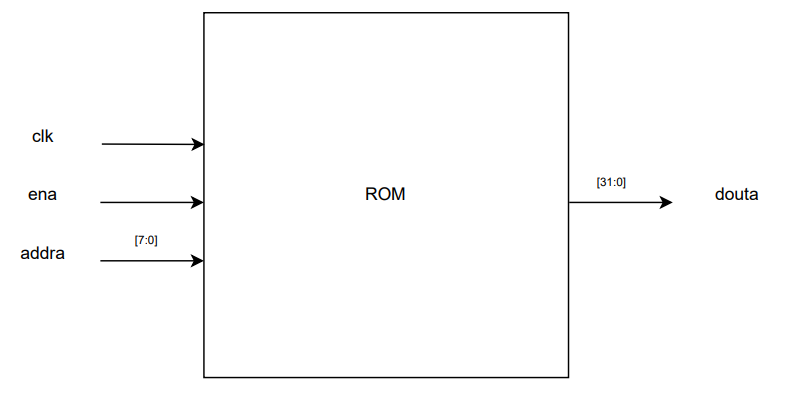
\includegraphics[width=0.6\textwidth]{./Images/img_implementacion_hw/diagramamoduloROM.png}
    \caption{Diagrama de la ROM que se usa en el filtrado de la señal}
    \label{fig:diagramamoduloROM}
\end{figure} 

\begin{figure}[h!]
    \centering
    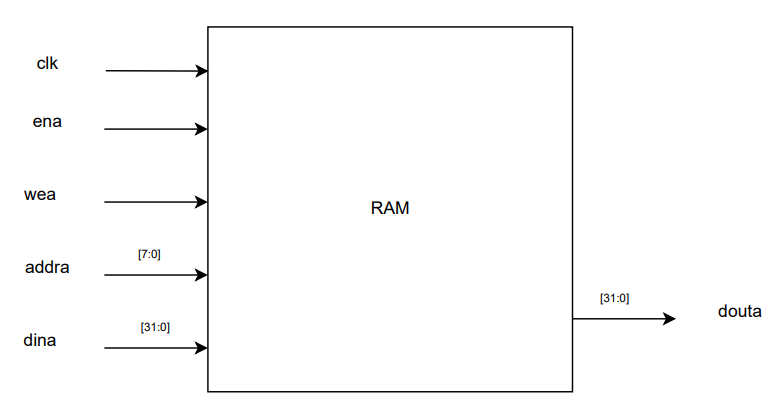
\includegraphics[width=0.6\textwidth]{./Images/img_implementacion_hw/diagramamoduloRAM.png}
    \caption{Diagrama de la RAM que se usa en el filtrado de la señal}
    \label{fig:diagramamoduloRAM}
\end{figure} 

\begin{figure}[h!]
    \centering
    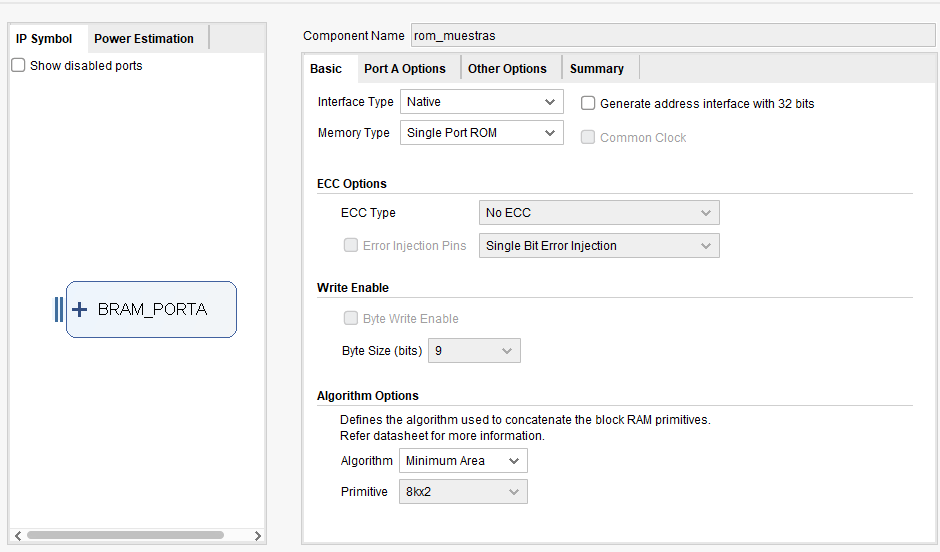
\includegraphics[width=0.6\textwidth]{./Images/img_implementacion_hw/rom_muestras_1.png}
    \caption{Selección de la opción simple port ROM}
    \label{fig:rom_muestras_1}
\end{figure}
 Es importante desactivar la opción de primitive output para que no se añada un registro extra 
 al principio y la simulación se ejecute en cada tiempo correspondiente. 
\begin{figure}[h!]
    \centering
    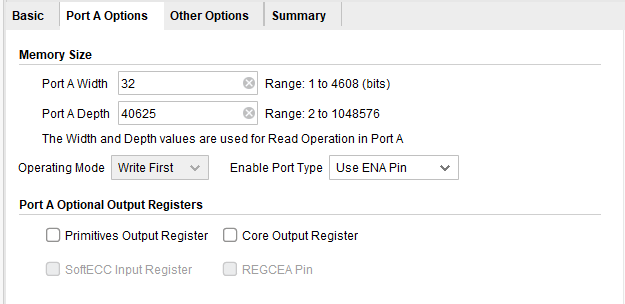
\includegraphics[width=0.6\textwidth]{./Images/img_implementacion_hw/rom_muestras_2.png}
    \caption{Se establece la profundidad de la ROM y la anchura de palabra}
    \label{fig:rom_muestras_2}
\end{figure}

El módulo de filtrado utiliza 1 ROM y una RAM

\begin{itemize}
\item La ROM se configura igual que la ROM del módulo de input, este tiene 99 filas y de anchura 
tiene 32 bits.
\item La RAM se configura como single port RAM y se mantiene desactivado el valor de primitive output.
 Ahora bien los valores asignados son los siguientes.
 
\begin{figure}[h!]
    \centering
    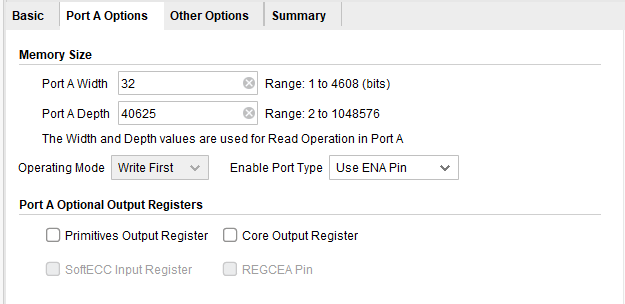
\includegraphics[width=0.6\textwidth]{./Images/img_implementacion_hw/rom_muestras_2.png}
    \caption{Se establece la profundidad de la RAM y la anchura de palabra}
    \label{fig:ram_muestras_1}
\end{figure}

\end{itemize}

\subsection{Módulos punto flotante}

Se han definido varios módulos para hacer las distintas operaciones en punto flotante, ya que en VHDL no se
pueden hacer estas operaciones directamente, se necesitan usar otros módulos especializados para estas operaciones.

Como se operan con valores en punto flotante simple, las señales tienen que ser de 32 bits.

En este programa se necesitan 5 tipos de módulos de operaciones.

\begin{itemize}
    \item Módulo comparador mayor que: se utiliza para comparar varias señales en el módulo de detección de picos como son:
    \begin{itemize}
        \item signal\_data gt last\_peak
        \item signal\_data gt cutoff
        \item last\_peak gt cutoff
    \end{itemize}

    \begin{figure}[h!]
        \centering
        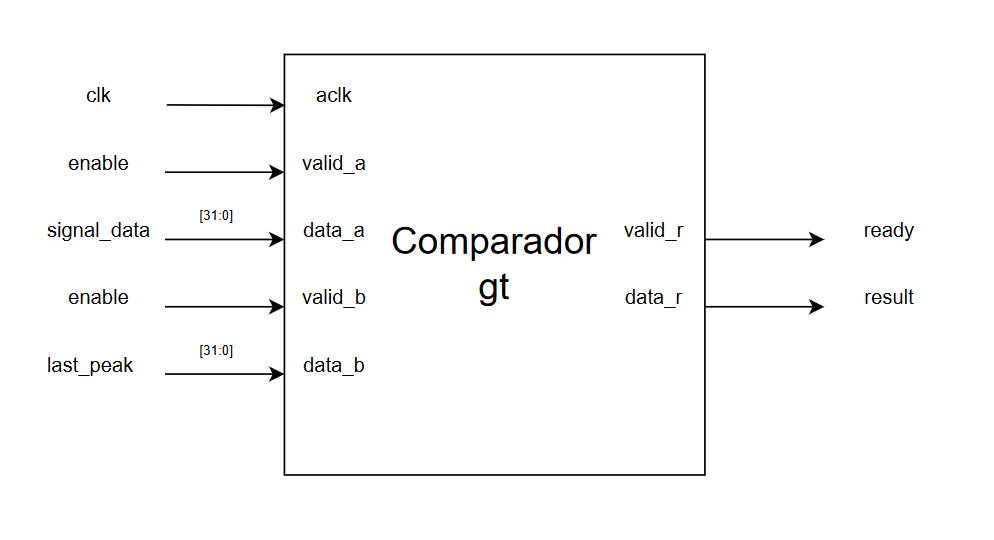
\includegraphics[width=0.8\textwidth]{./Images/img_implementacion_hw/comparadorgt.png}
        \caption{Entrada y salida del módulo de comparador}
        \label{fig:comparadorgt}
    \end{figure}

    \item Módulo divisor y resta: se utilizan en conjunto para calcular el cutoff que tiene la operacion:
    \[cutoff = cutoff - cutoff/192\]

    \begin{figure}[h!]
        \centering
        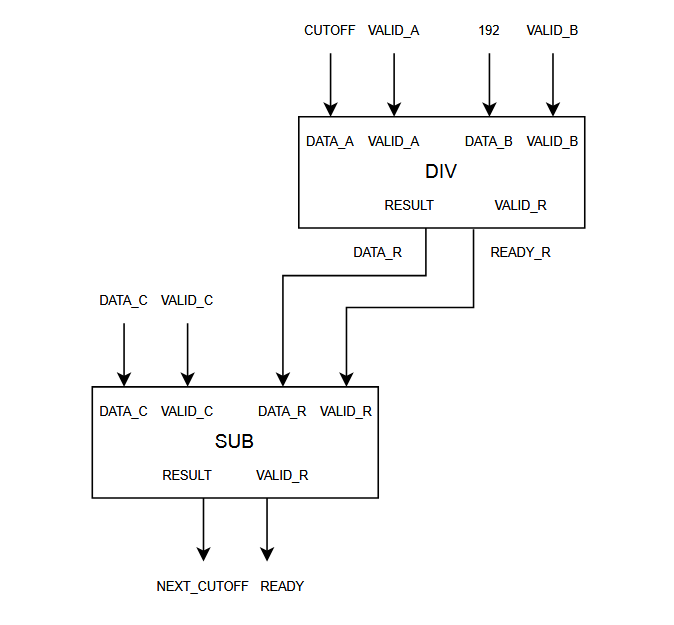
\includegraphics[width=0.6\textwidth]{./Images/img_implementacion_hw/DiagramaDivisorrestador.png}
        \caption{Funcionamiento de la conexión de los módulos de divisor y restador}
        \label{fig:divisorrestador}
    \end{figure}   

    \item Módulo multiplicación y suma: Se usa para poder multiplicar los valores de las muestras con los valores de los coeficientes en el módulo de filtrado.
    \begin{figure}[h!]
        \centering
        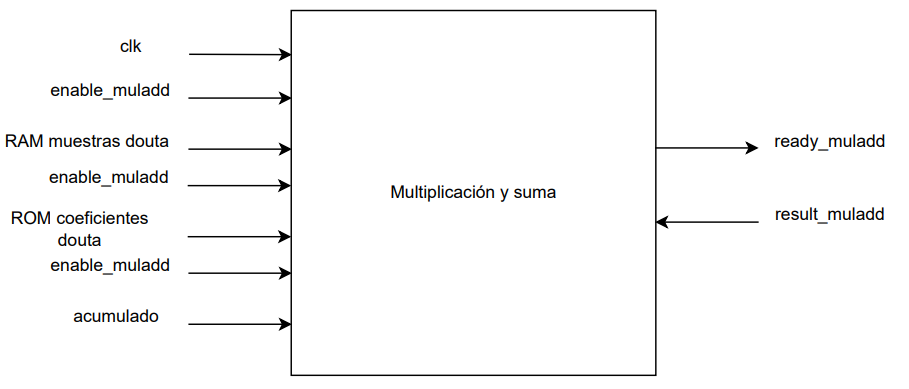
\includegraphics[width=0.6\textwidth]{./Images/img_implementacion_hw/diagramamodulomultiplicacionysuma.png}
        \caption{Diagrama de Módulo de multiplicación y suma.}
        \label{fig:diagramamodulomultiplicacionysuma}
    \end{figure}
\end{itemize}

\section{Módulo de filtrado}

Este módulo utiliza una ROM con los coeficientes, una RAM con las muestras y un módulo de multiplicación
de números en punto flotante.

Este módulo se compone de una máquina de estados que va multiplicando cada elemento de la RAM muestras 
con los elementos de la ROM coeficientes con el módulo de multiplicación de punto flotante.

\subsection{Señales de entrada y salida}

Las señales de entrada son:

\begin{itemize}
\item clk y reset
\item input\_signal\_data: señal que recibe las muestras de la señal original 
\item input\_valid e input\_ready: son flags que sirven para sincronizar el módulo con la llegada de muestras. 
\end{itemize}

Las señales de salida son:

\begin{itemize}
    \item output\_filter\_data: saca los valores de la señal filtrada
    \item output\_filter\_index: saca los índices de cada valor de la señal filtrada
    \item output\_valid y output\_ready: se encargan de sincronizar el módulo del filtrado 
    con el módulo de detección de picos
\end{itemize}

\begin{figure}[h!]
    \centering
    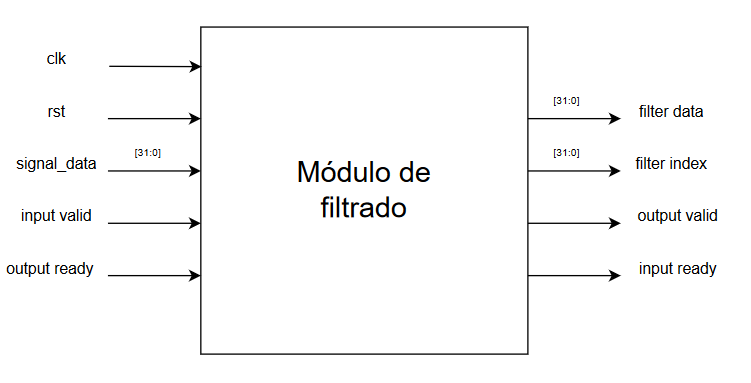
\includegraphics[width=0.6\textwidth]{./Images/img_implementacion_hw/diagramamodulofiltrado.png}
    \caption{Entradas y salidas del módulo de filtrado}
    \label{fig:modfiltrado}
\end{figure} 

\subsection{Máquina de estados}

\begin{figure}[h!]
    \centering
    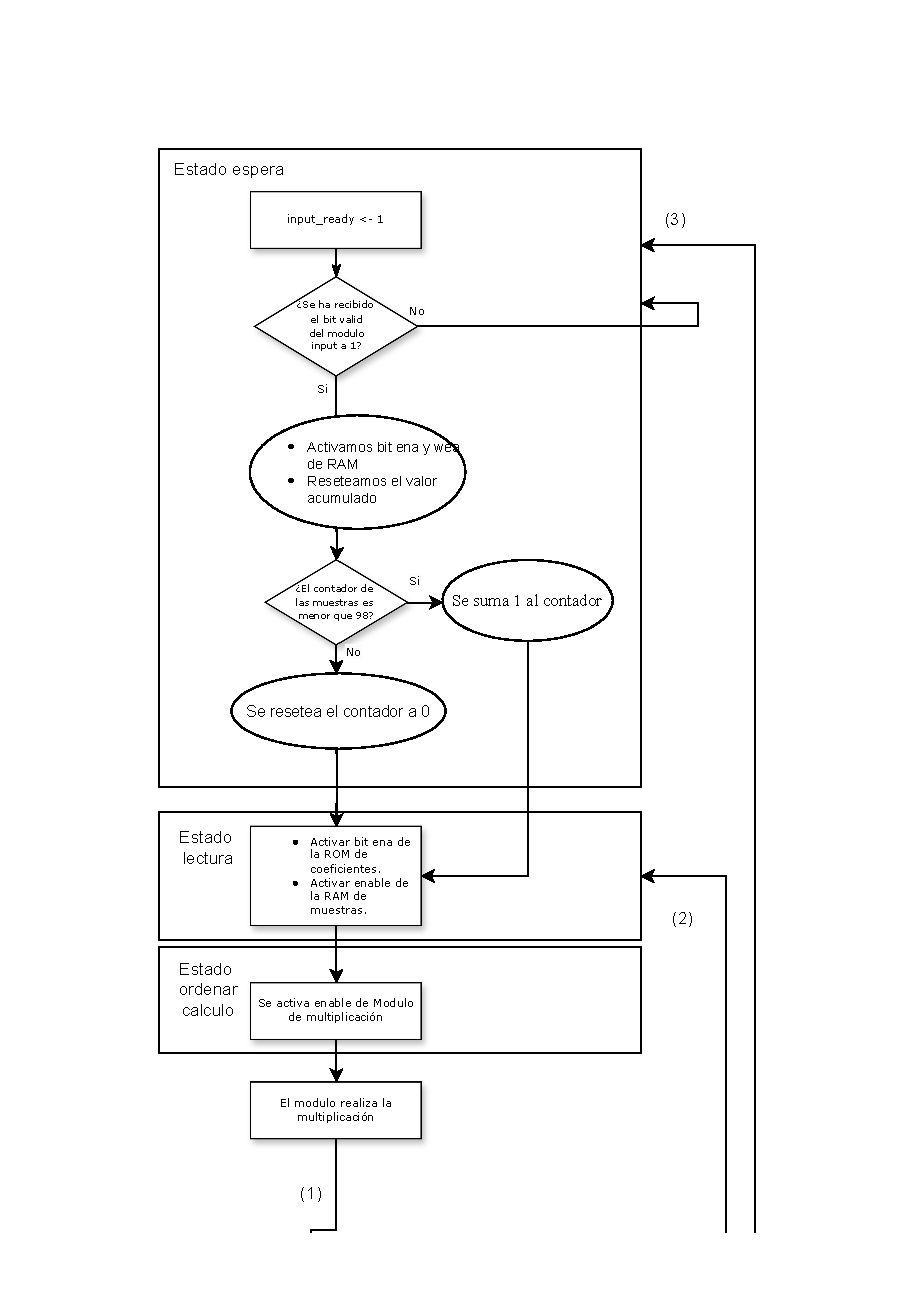
\includegraphics[width=0.99\textwidth]{./Images/img_implementacion_hw/Diagramaasmfiltrado1.pdf}
    \caption{Diagrama ASM de Módulo de filtrado de señal}
    \label{fig:Diagramaasmfiltrado1}
\end{figure} 

\begin{figure}[h!]
    \centering
    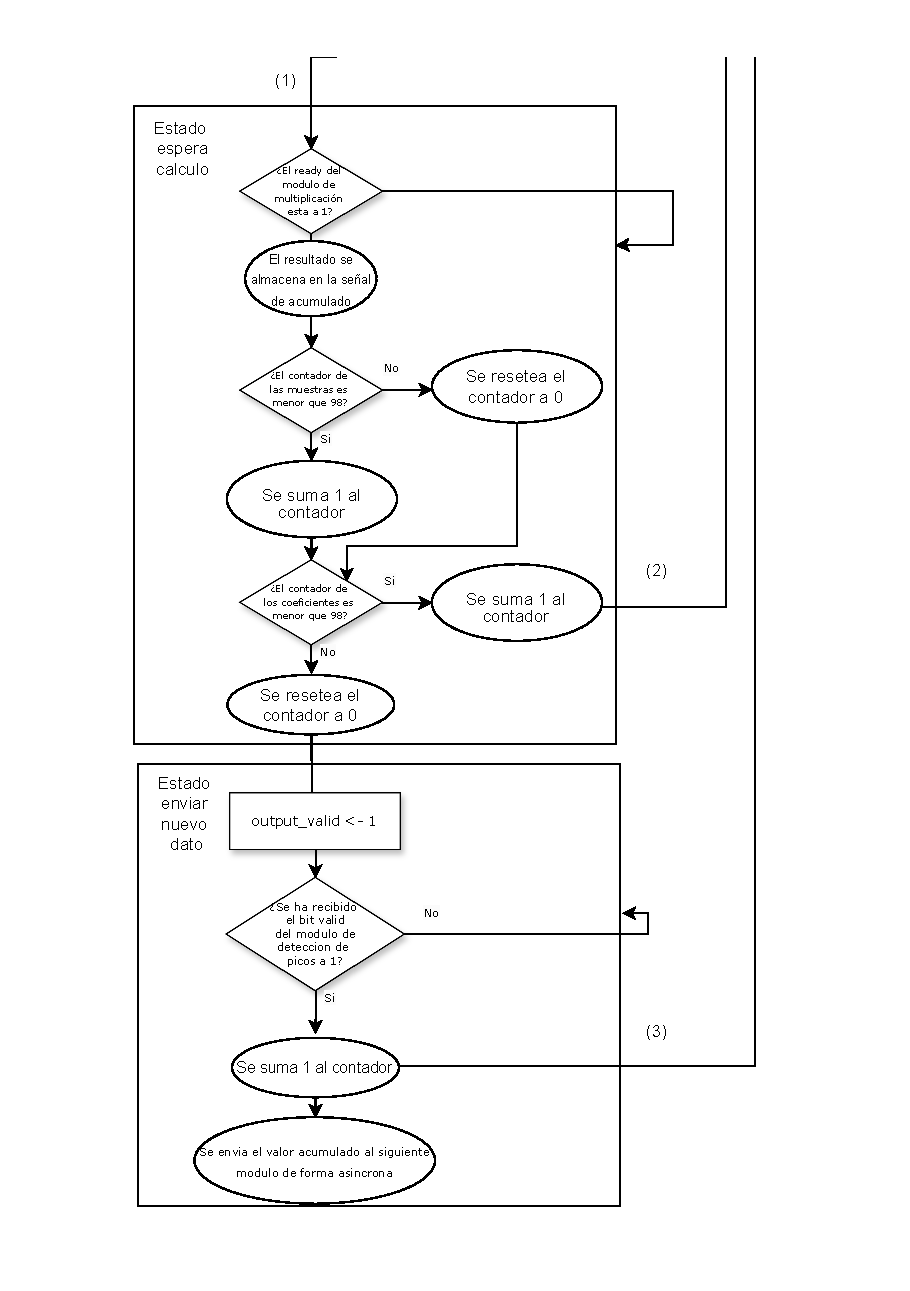
\includegraphics[width=0.99\textwidth]{./Images/img_implementacion_hw/Diagramaasmfiltrado2.pdf}
    \caption{Diagrama ASM de Módulo de filtrado de señal}
    \label{fig:Diagramaasmfiltrado2}
\end{figure} 
\FloatBarrier
El envio de datos al output se realiza de forma combinacional, se pasa a \lstinline{output_data} el 
valor del acumulado y el índice a su respectivo output.
\begin{itemize}
    \item Estado de espera: En el estado de espera se activa la señal de ready y se espera a que se envie un valor de la
    señal sin filtrar, se borra el valor de la solución de la multiplicación anterior en caso de haberla, se activan las
    señales de escritura de la RAM y se establece el índice donde se va a escribir la muestra.
    \item Estado de lectura: Se activa la lectura de los coeficientes y de las muestras.
    \item Estado para ordenar el cálculo: en este estado se activa el flag del módulo de multiplicacion.
    \item Estado de espera del cálculo: se espera a que termine el módulo de multiplicacion esperando la señal de ready\_muladd
    y se almacena el resultado, tambien se actualiza el contador de los coeficientes, de las muestras y dependiendo de si el 
    índice de coeficientes es menor que 98 se va al estado de lectura o el estado de enviar un nuevo dato al siguiente módulo.
    \item Estado de envio de nuevo dato: este estado sincroniza el siguientemódulo, activa el bit de valid a 1 y espera el bit
    de ready del siguiente módulo para poder enviar el dato.
\end{itemize}

\subsection{Módulos utilizados}
Se utilizo una ROM para almacenar los coeficientes y poder leerlos y una RAM 
para poder leer y escribir en las muestras de la señal original.

Se usa un módulo de multiplicación para poder multiplicar los valores de las muestras con los valores de los coeficientes.

\section{Módulo de detección de picos}

Este módulo se encarga de detectar los picos de la señal filtrada. 
\subsection{Señales de entrada y salida}

    \begin{figure}[h!]
        \centering
        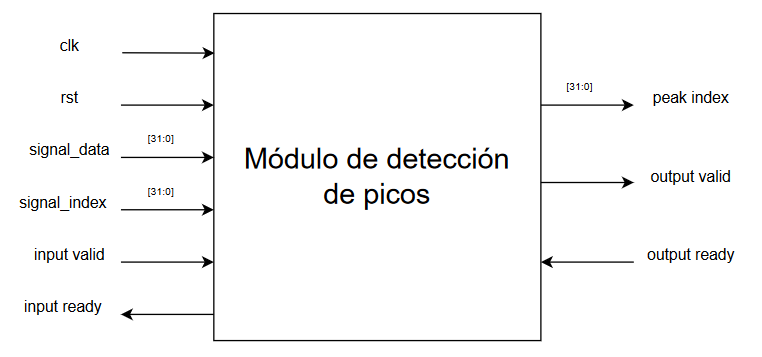
\includegraphics[width=0.6\textwidth]{./Images/img_implementacion_hw/diagramamodulodeteccionpicos.png}
        \caption{Entradas y salidas del módulo de detección de picos}
        \label{fig:moddeteccionpicos}
    \end{figure} 
    
    \begin{itemize}
    \item clk y reset
    \item input\_signal\_data: señal que recibe las muestras de la señal filtrada 
    \item input\_signal\_index: señal que recibe los índices de las muestras de la señal filtrada 
    \item input\_valid e input\_ready: son flags que sirven para sincronizar el módulo con la llegada de muestras. 
    \end{itemize}
    
    Las señales de salida son:
    
    \begin{itemize}
        \item output\_peak\_index: saca los índices de los picos detectados
        \item output\_valid y output\_ready: Se encargan de sincronizar el módulo de deteccion de picos 
        con el módulo de deteccion de arritmias.
    \end{itemize}

\subsection{Máquina de estados}

\begin{itemize}
    \item Estado de espera: En el estado de espera se activa la señal de ready y se espera a que se envie un valor de la
    señal sin filtrar, se borra el valor de la solucion de la multiplicacion anterior en caso de haberla, se activan las
    señales de escritura de la RAM y se establece el indice donde se va a escribir la muestra.
    \item Estado de comprobar indice: si no hay pico, o lo que es lo mismo que la señal de last\_peak este a 0 este se asigna
     a la señal y ademas se registra el indice, despues pasa al estado de actualizar el cutoff activando por tanto la señal de 
     division para que empiecen los módulos de division y resta de valores en punto flotante a calcular el valor. Si por otro
     lado si que hay pico, se ordena hacer la comparación \lstinline{signal_data > last_peak} pasando las señales correspondientes al módulo de comparacion en 
     punto flotante. Además se anticipa y se hace la comparación \lstinline{last_peak > cutoff} para en dado caso de que no se cumpla la 
     condicion anterior ya esta la comparacion hecha y se pude pasar directamente al estado siguiente. Tambien activamos las señales
     del módulo de comparacion correspondiente. El siguiente estado es el estado de espera a la condicion en la que la señal es mayor 
     que el pico maximo.
    \item Estado de actualizar cutoff: este estado espera a la señal ready del módulo de la resta ya que es la ultima operacion que se realiza para 
    calcular el cutoff. Primero se ejecuta el módulo de la division para calcular cutoff/192 y luego la resta cutoff - cutoff/192. cuando la señal
    ready\_sub sea '1' se actualiza el cutoff y pasa al estado de espera terminando la iteracion. 
    \item Estado de espera a la condicion en la que la señal es mayor que el pico maximo: cuando las señales ready de los comparadores esten a '1' 
    se podra ejecutar las funcionalidades del estado. este tiene 3 condiciones:
    \begin{itemize}
        \item si se ha encontrado un valor mas alto que last\_index, este pico pasa a ser el nuevo last\_peak y el nuevo cutoff, el index tambien se actualiza. 
        \item la señal result\_signal\_index\_sub\_last\_index\_gt\_or\_eq\_samples\_around\_peak se calcula de forma combinacional, por lo que si esa condicion que
         indica que han pasado 72 muestras sin encontrar un valor mas alto que last\_peak y ademas last\_peak es mayor que el cutoff, se pasa directamente al estado
         de envio de nuevo pico para enviar el pico QRS.
        \item Sino simplemente se ordena la actualizacion del cutoff activando el enable del módulo de la division y pasando al estado correspondiente.
    \end{itemize}
    \item Estado de envio de nuevo pico: se activa la señal de valid a 1 y espera a que el módulo de deteccion de arritmias mande la señal de ready para resetear 
    las señales de last peak y last index a '0' ademas se actualiza el cutoff.
\end{itemize}

\begin{figure}[h!]
    \centering
    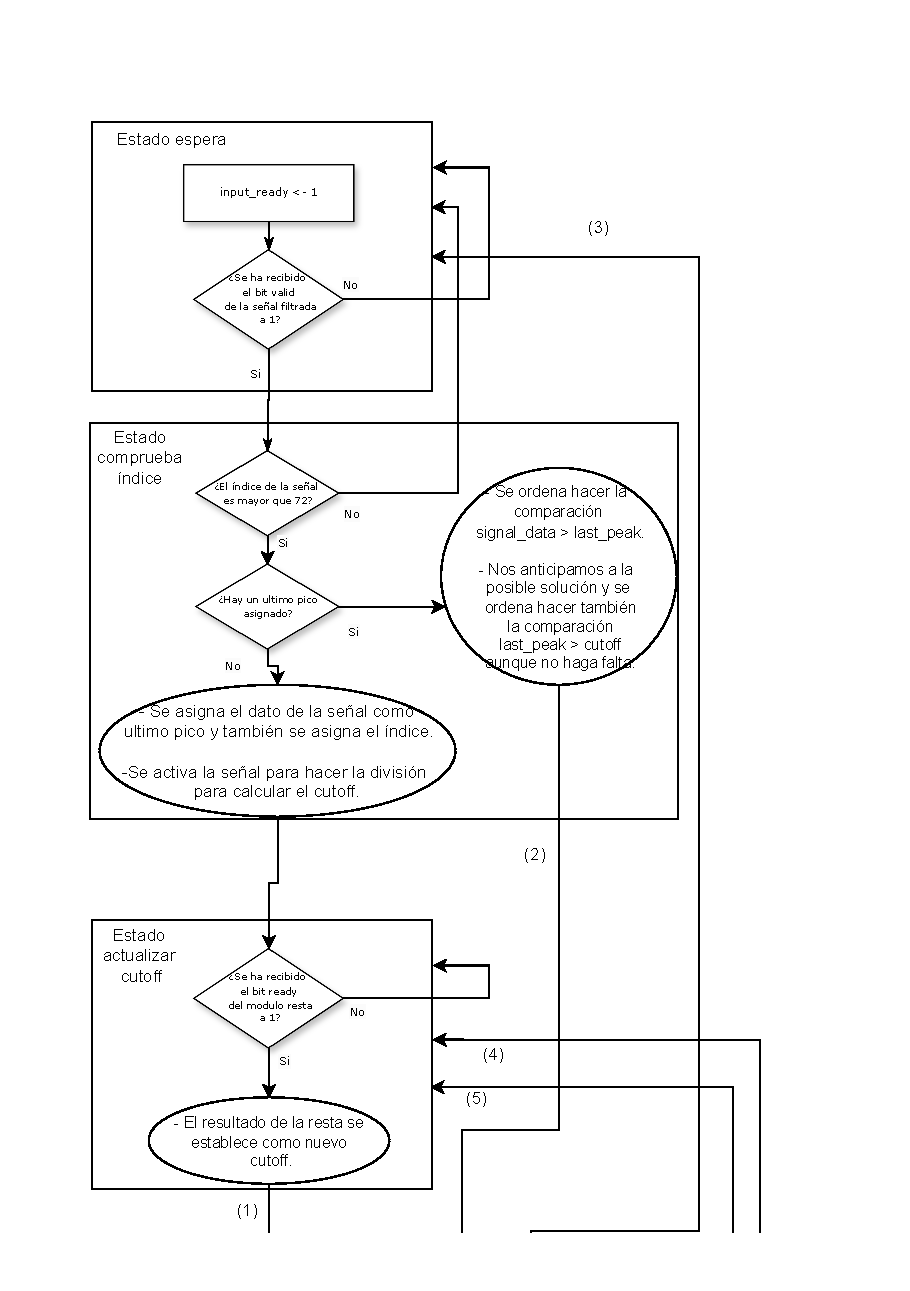
\includegraphics[width=0.99\textwidth]{./Images/img_implementacion_hw/Diagramaasmpicos1.pdf}
    \caption{Diagrama ASM de Módulo de detección de picos}
    \label{fig:Diagramaasmpicos1}
\end{figure} 

\begin{figure}[h!]
    \centering
    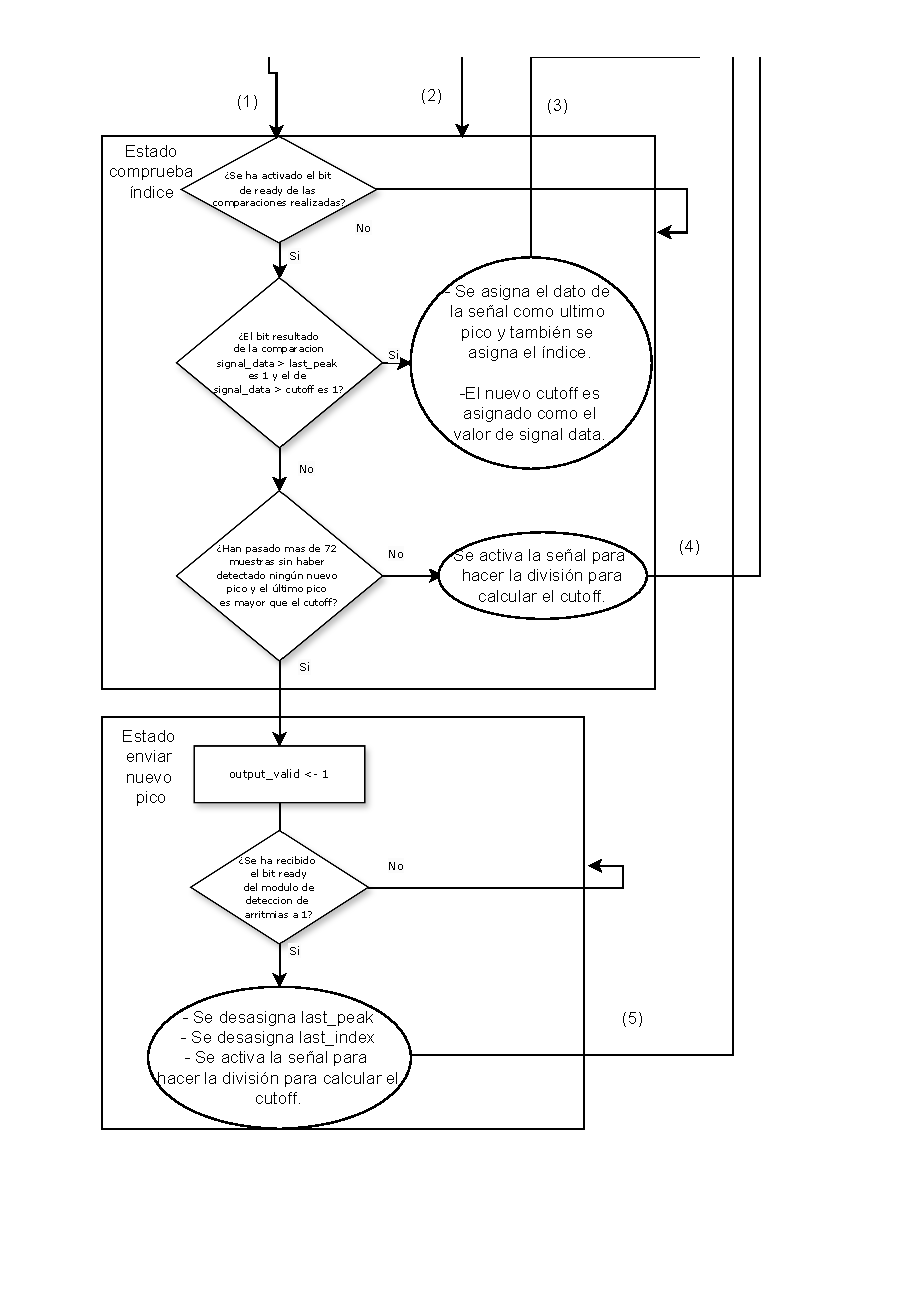
\includegraphics[width=0.99\textwidth]{./Images/img_implementacion_hw/Diagramaasmpicos2.pdf}
    \caption{Diagrama ASM de Módulo de detección de picos}
    \label{fig:Diagramaasmpicos2}
\end{figure} 
\FloatBarrier
De manera combinacional se pasa como output last index pero el módulo de deteccion de arritmias se activa cuando input\_valid
se activa usando así el \lstinline{last_index} correspondiente 


\section{Módulo de detección de arritmias}

El módulo de detección de arritmias se encarga de detectar si la distancia entre 2 picos QRS es considerada una arritmia o no,
 
\subsection{Señales de entrada y salida}
Las señales de entrada de este módulo son:

\begin{itemize}
    \item clk y reset
    \item input\_peak\_index: señal que recibe las muestras de los picos QRS.
    \item input\_valid e input\_ready: son flags que sirven para sincronizar este módulo con el módulo de deteccion de picos. 
\end{itemize}
    
Las señales de salida son:

\begin{itemize}
    \item output\_arrythmia\_detected: flag que saca 0 si el ritmo es normal y 1 si se ha detectado una arritmia.
    \item output\_arrythmia\_index: valor que indica en que sample se ha producido la arritmia.
    \item output\_valid y output\_ready: para la sincronización con el módulo output.
\end{itemize}

\begin{figure}[h!]
    \centering
    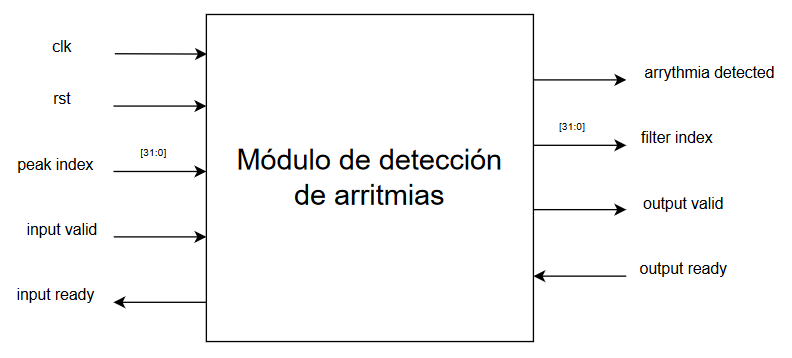
\includegraphics[width=0.6\textwidth]{./Images/img_implementacion_hw/diagramamodulodeteccionarritmias.png}
    \caption{Entradas y salidas del módulo de detección de arritmias}
    \label{fig:moddeteccionarritmias}
\end{figure} 

\subsection{Máquina de estados}

\begin{itemize}
    \item Estado de espera: En el estado de espera se activa la señal de ready y se espera a que se envie un pico QRS, despues pasa al estado S0
    \item Estado S0: Si el contador es 0 significa que se recibe el primer pico registrado por lo que se guarda para mas tarde y se pasa al estado de espera.
    Si el contador es 1 significa que se recibe el segundo pico y por tanto se compara con el anterior hallando la primera distancia despues pasa al estado S1.
    Si no se cumple ninguna condición se pasa al estado S1.    
    \item Estado S1: aumenta el contador en 1, y se calcula la distancia actual.
    \item Estado S2: se actualizan las variables que crean un buffer ficticio y los valores se mueven una posicion cuando se añade la distancia actual como si fuese una cola.
    \item Estado S3: Como ya se explicó en la parte de la implementación del algoritmo TNRange es una señal que simbiliza la distancia entre el pico detectado como arritmia y 
    el pico normal actual, este flag se activa cuando ha habido una arritmia ya que last\_distance puede ser mas grande de lo normal, es por eso que para calcular el gap cuando este flag esta activo
     y el de arritmia detectada no, se compara la distancia actual con la ultima distancia sino con una 3 veces anterior a la última. Si esta condicion no se cumple, para calcular el gap se compara 
     con la ultima distancia, además si justo la anterior distancia era la de una arritmia, se desactiva el flag de arritmia detectada.
    \item Estado S4: Se calcula el procentaje de forma combinacional, si el flag de porcentaje es igual a 1 significa que el porcentaje calculado es mayor de lo esperado y por tanto se activan las flags
    de TNRange y counter\_arrythmias. Independientemente despues el indice y la distancia actual pasan a ser last\_distance y last\_index
    \item Estado S5: Se activa la señal de valid y se espera a la señal de ready para que se envie el dato al módulo de output.
\end{itemize}

Se calcula el porcentaje del gap entre las 2 distancias con una distancia normal de forma combinacional.

\begin{itemize}
    \item Estas señales estan en complemento A2 por ello al salir numeros negativos, el bit mas significativo se cambia a 1, es por ello que como solo se consideran los numeros positivos, se
     considera solamente los numeros cuyo bit mas significativo sea 0
    \item como al principio la señal de la ultima distancia es x"00000000" al comparar esta distancia con la actual saldra una distancia enorme que activara el bit del porcentaje que se calcula 
    de forma combinacional asiq ue quitramos ese caso especifico de por medio.
    \item en vez de hacer una division del gap entre distance\_for\_calc se sigue esta fórmula:
    \[ gap/distanceforcalc > 0.15\] 
    \[gap > 0.15 \cdot distanceforcalc \] 
    \[gap > distanceforcalc>> 5 + distanceforcalc>> 3 + distanceforcalc\] 
\end{itemize}

\lstset{language=VHDL, breaklines=true, basicstyle=\footnotesize}
\begin{lstlisting}[frame=single]
    percentage <= '1' when gap(31) = '0' and last_distance > x"00000000" and (std_logic_vector(shift_right(unsigned(distance_for_calc), 3) + shift_right(unsigned(distance_for_calc), 5)) <= std_logic_vector(unsigned(gap))) else '0';
\end{lstlisting}


\begin{figure}[h!]
    \centering
    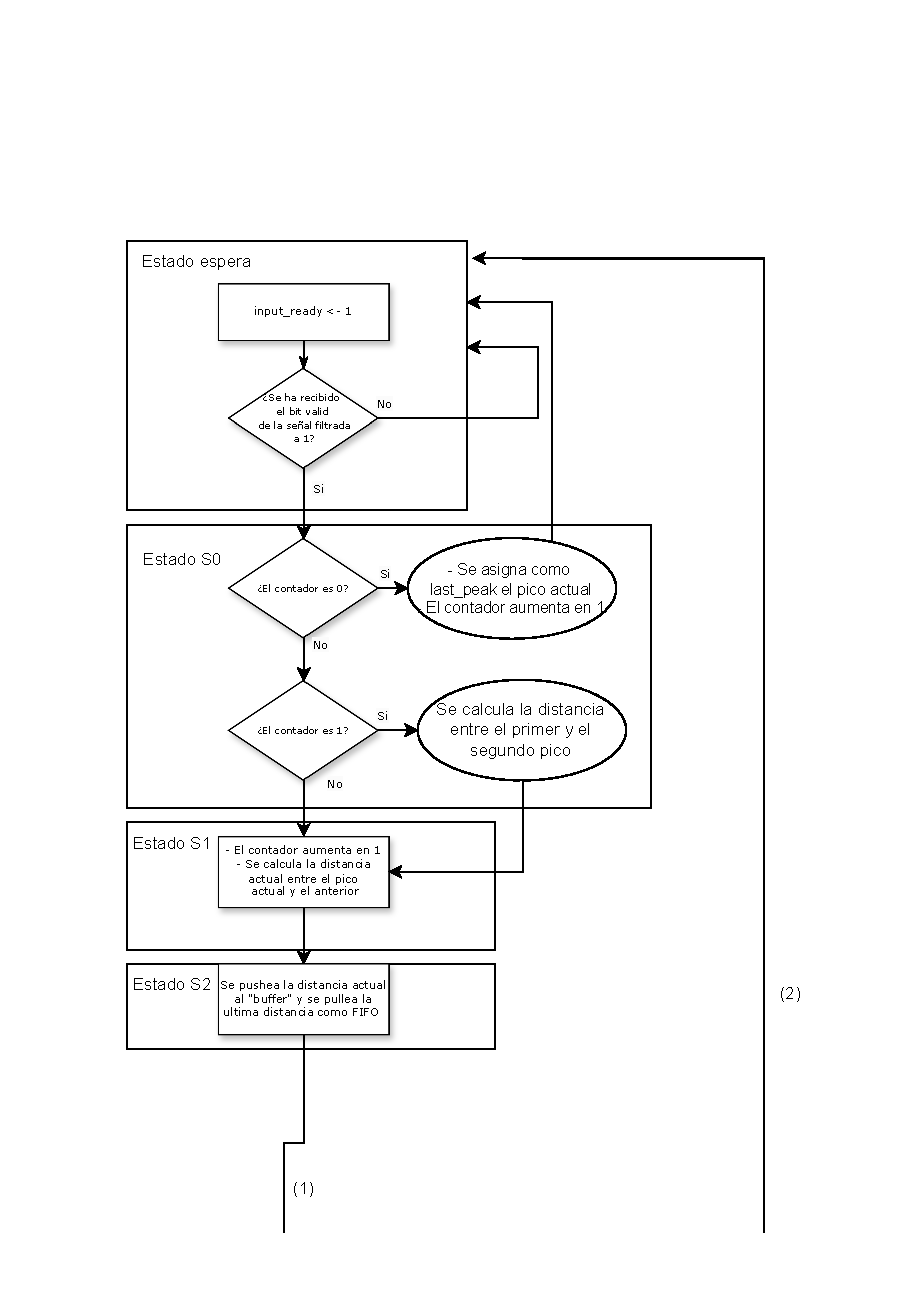
\includegraphics[width=0.99\textwidth]{./Images/img_implementacion_hw/Diagramaasmarritmias1.pdf}
    \caption{Diagrama asm de Módulo de filtrado de señal}
    \label{fig:Diagramaasmarritmias1}
\end{figure} 

\begin{figure}[h!]
    \centering
    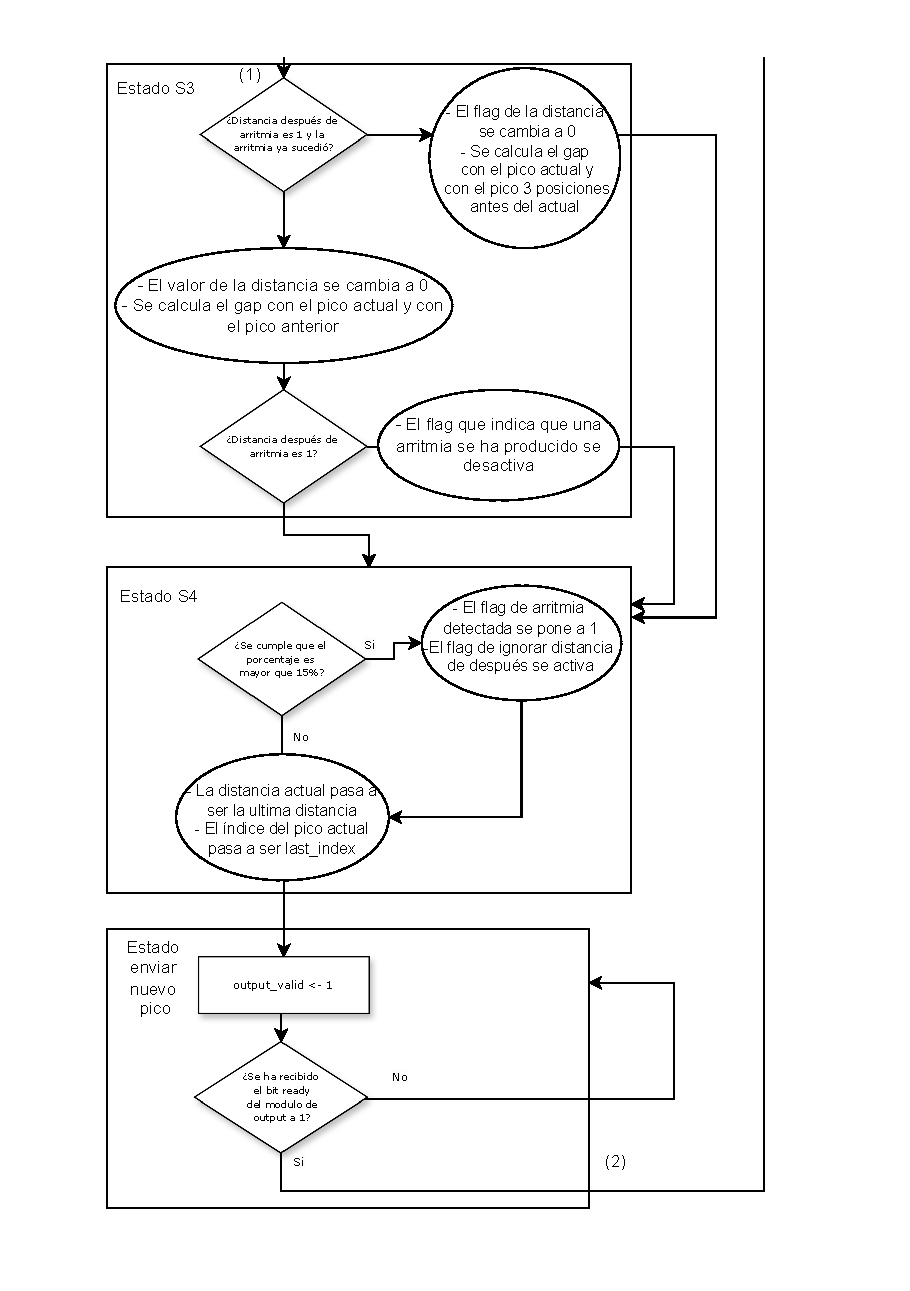
\includegraphics[width=0.99\textwidth]{./Images/img_implementacion_hw/Diagramaasmarritmias2.pdf}
    \caption{Diagrama asm de Módulo de filtrado de señal}
    \label{fig:Diagramaasmarritmias2}
\end{figure} 
\FloatBarrier
\section {Módulos input y output}
Estos módulos se componen de un estado de lectura y uno de escritura donde uno lee el dato y el otro se encarga de esperar a que se lea el dato y actualizar 
el contador para que se pueda leer de la siguiente posicion de la ROM

\subsection{Módulo input}
\begin{itemize}
    \item Estado de lectura: Primero se asegura de que el contador no hay llegado a la cantidad de muestras máximas en este caso 40625, después pone el bit de enable a 1 
    y pasa al estado de espera.
    \item Estado de espera: pone el bit de valid a 1 y espera al bit de ready para que el siguiente módulo lea el dato, actualiza el contador y pasa al estado de lectura.
\end{itemize}

Este módulo cuenta con una ROM con los valores de la señal original, valores que se van leyendo cundo la señal de ready se activa.

\subsection{Módulo output}
\begin{itemize}
    \item Estado de lectura: Primero se asegura de que el contador no hay llegado a la cantidad de muestras máximas en este caso 144, después pone el bit de enable a 1 
    y pasa al estado de espera. Si se han leido todas las muestras pasa al estado correcto.
    \item Estado de espera: pone el bit de valid a 1 y espera al bit de ready para que el siguiente módulo lea el dato, actualiza el contador y se comprueba si la anotacion
    del pico coincide con la anotacion de la BRAM que es la anotacion original. Ademas se asegura que la anotacion pertenece al indice correcto, si esta condicion se cumple
    sigue con la ejecucion, si no pasa al estado de error.
    \item Estado error: pone la señal de error a 1 y se para la ejecucion ya que un resultado no coincide.
    \item Estado correcto: pone la señal de correcto a 0 que indica que el programa ha sido replicado con exito.
\end{itemize}

Este módulo cuenta con una ROM con las anotaciones de los cardiologos de casa pico QRS, valores que se van leyendo cundo la señal de valid se activa.

\section{Módulo principal y testbench}

El módulo principal se encarga de sincronizar los módulos pasando los datos de un módulo al siguiente asi como la señal de valid y transferir de vuelta la señal de ready.

Tambien se ha definido un testbench donde se definen los ciclos de reloj, ademas del reset al principio de la ejecucion. Como salida tiene los estados correcto y error para 
ver los resultados de la ejecucion.



	\chapter{Resultados Experimentales}


\section{Entorno de pruebas}
Para hacer las pruebas en la placa se ha utilizado la Basys3 de virtex ya que se utiliza la misma en el estudio en el que se basa el proyecto.

El problema que se encontró con el uso de la placa es que la ROM no podría almacenar 650000 filas de valores de punto flotante por lo que se probo un dieciseisavo de las pruebas totales que equivale a 40625.

Por lo que, para hacer la prueba con todos los samples, se requiere utilizar una FPGA con mas recursos como la Virtex-7 VC709 Evaluation Platform.

\begin{figure}[h]
	\centering
	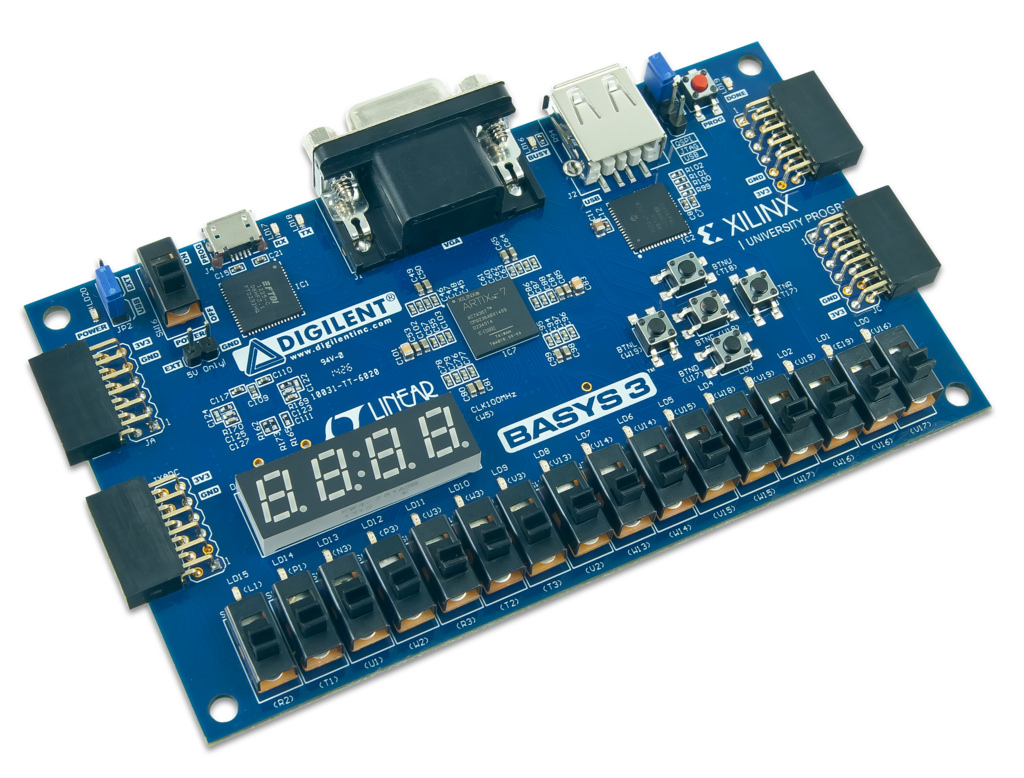
\includegraphics[width=0.6\textwidth]{./Images/img_introduccion/Basys3.jpg}
	\caption{Basys3 Artix-7 FPGA}
	\label{fig:Basys3}
\end{figure}

\section{Consumo}
	Para evaluar el consumo se tendrá en cuenta los resultados sacados del análisis de síntesis, del reporte de timing y de el reporte de potencia de el modulo principal que contiene el modulo de filtrado de señal,
	el módulo de deteccion de picos y el modulo de deteccion de arritmias. 
	
	\begin{figure}[h!]
		\centering
		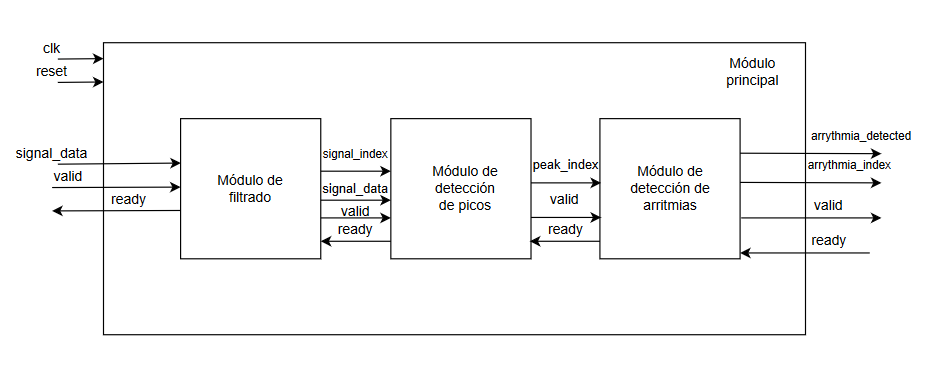
\includegraphics[width=0.99\textwidth]{./Images/img_res_experimentales/diagramaGeneral.png}
		\caption{Diagrama principal de todos los módulos a evaluar}
		\label{fig:Diagramaasmfiltrado}
	\end{figure} 

\FloatBarrier

\subsection{Análisis de síntesis}

	En el análisis de síntesis podemos ver las siguientes caracteristicas:

	\begin{itemize}
		\item Luts as logic: 195
		\item Luts as memory: 0
		\item Slice registers: Hay 279 slice registers de los cuales todos son flip flops y no hay ningun latch por la arquitectura 
		seguida en la creacion del programa haciendo que al pasar de estado se cambien todas las señales nuevas por las actuales
		\item No se ha usado ningún DSP
		\item No se ha usado ninguna block RAM tile
		\item Hay un total de 474 total slices
		\item La frecuencia de funcionamiento configurada en el .xdc es de 640800 pero para las pruebas se usara una frecuencia de 540000
	\end{itemize}

	La frecuencia de funcionamiento se ha calculado segun la referencia de el articulo \cite{desai2021low} que nos indica que las muestras van a 360sps (samples per second) 
	por lo que es equivalente a 360Hz. Tambien se calcula el numero de ciclos que tarda en ejecutarse el modulo de filtrado que resulta ser el mas critico 
	de todos, este da un total de 1780 ciclos pero para hacer las pruebas se usaran 1500 ciclos. Si se multiplican ambos valores da una frecuencia de 540000 
	cuyo periodo es de 1851,85 que redondeando es de 1852. En el xdc se pone lo siguiente:

\lstset{language=VHDL, breaklines=true, basicstyle=\footnotesize}
\begin{lstlisting}[frame=single]
## Clock signal
set_property PACKAGE_PIN W5 [get_ports clk]							
	set_property IOSTANDARD LVCMOS33 [get_ports clk]
	create_clock -add -name sys_clk_pin -period 1852.00 -waveform {0 926} [get_ports clk]
\end{lstlisting}

El waveform oscila desde 0 a 926 para que sea simétrico.

\subsection{Análisis de timing}
	En el análisis de timing se vera cual es el worst negative slack y se calculara la frecuencia minima necesaria. Este reporte de timing muestra lo siguiente.

	\begin{figure}[h!]
		\centering
		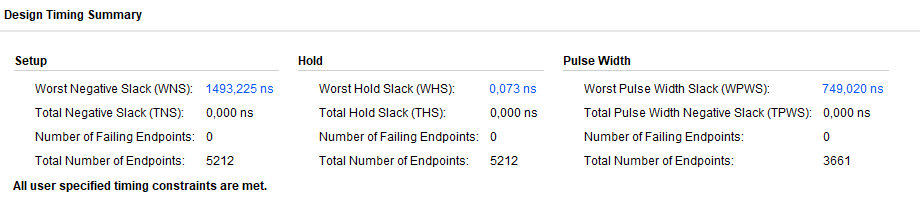
\includegraphics[width=0.9\textwidth]{./Images/img_res_experimentales/reportetiming.png}
		\caption{Imagen que muestra el reporte de timing generado}
		\label{fig:reporteTiming}
	\end{figure} 

	Para calcular la frecuencia minima necesaria se resta la frecuencia actual menos el worst negative slack dando como resultado 6,49 ns de frecuencia mínima de funcionamiento. 

\subsection{Análisis de potencia}

	En el análisis de potencia se evalua la potencia que necesita la FPGA para poder llevar a cabo las instrucciones.

	\begin{figure}[h!]
		\centering
		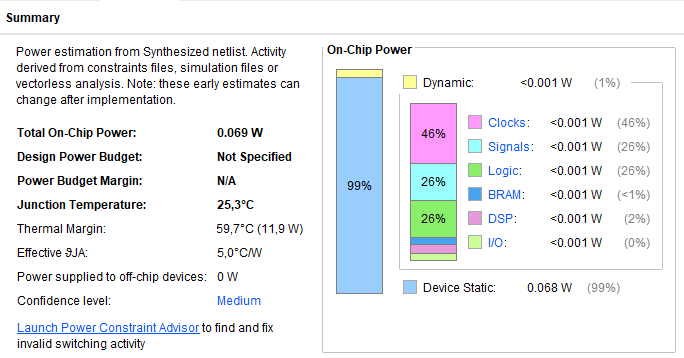
\includegraphics[width=0.6\textwidth]{./Images/img_res_experimentales/reportepower.png}
		\caption{Imagen que muestra el reporte de potencia generado}
		\label{fig:reportepotencia}
	\end{figure} 

	Comparando este proyecto con otros estudios, por ejemplo con el de caracterizacion de señales usando polinomios de hermite presentan unos resultados de dynamic potencia de 28mW.
	Sin embargo, el dynamic potencia de este proyecto es menor que 0,001W.








	
	\chapter*{Conclusión}
Este proyecto trata de buscar una solución simple para la detección de 
arritmias de una señal de un electrocardiograma, Para la elaboración de este proyecto, 
se ha estudiado el comportamiento de las arritmias, viendo la base de datos de MIT y estudiando
el comportamiento de las arritmias anotadas se observó que la inmensa mayoría de las arritmias 
que ocurrían eran dadas por una contracción prematura del corazón, por tanto el proyecto, aunque
inicialmente se pensó detectar el mayor tipo de arritmias posibles, al no ver ningún ejemplo claro
de arritmia no producida por una contracción prematura el proyecto solo se centró en detectar dichas arritmias.

Se realizó un prototipo en python que sirvió para crear el algoritmo y probarlo con facilidad. Este prototipo inicia
con un filtrado de la señal original aplicando el filtrado FIR. Seguidamente se aplica un algoritmo de detección de 
picos QRS sobre la señal filtrada que busca el pico más alto que además sobrepase el cutoff dinámico establecido. Finalmente
se aplica el algoritmo de detección de arritmias calculando la distancia entre el pico actual con el anterior y comparándola con una
distancia anterior de un ritmo normal.

Para la implementación de hardware se usarán 3 módulos principales que son el módulo de filtrado, el módulo de detección de picos 
y el módulo de detección de arritmias. Además estos módulos están contenidos en un módulo principal. Para hacer las pruebas sobre
estos módulos, se añaden 2 módulos adicionales de input de señal y output donde se comparan los resultados de las anotaciones. Además 
se evalúan los resultados mediante una simulación al crear un testbench.

Para las pruebas en hardware se utiliza la FPGA Virtex 7 en la placa Basys3, ya que es la FPGA que se usa en el estudio y aunque no sea capaz de 
albergar los 30 minutos de pruebas en la RAM, con menos pruebas tiene un buen desempeño.

En el fichero .xdc se ha establecido un periodo específico teniendo en cuenta la frecuencia de las muestras que es de 365 sps y da un periodo 
de 1852 ns. Gracias al reporte de timing se halla que la mínima frecuencia de funcionamiento es de 6,49 ns.

Según el reporte de potencia el consumo de la placa es de 0,069 W lo que resulta en un consumo bajo incluso para un uso continuo de este.
Comparándolo con otros proyectos similares, el consumo dinámico es menor.

\chapter*{Conclusion}

This project tries to find a simple solution for the detection of arrhythmias from an electrocardiogram signal. 
arrhythmias from an electrocardiogram signal. For the elaboration of this project, 
the behavior of the arrhythmias has been studied, looking at the database of MIT and studying the behavior of the
the behavior of the noted arrhythmias, it was observed that the vast majority of the arrhythmias that occurred 
the vast majority of the arrhythmias that occurred were due to premature contraction of the heart.
initially intended to detect as many arrhythmias as possible, but did not see any clear examples of arrhythmias not caused by premature
of arrhythmia not caused by premature contraction, the project only focused on detecting these arrhythmias.

A prototype was made in Python which was used to create the algorithm and test it easily. This prototype starts
with a filtering of the original signal by applying the FIR filtering. Next, a QRS peak detection algorithm is applied to the filtered signal. 
QRS peak detection algorithm is then applied to the filtered signal to find the highest peak that also exceeds the established dynamic cutoff.
Finally, the arrhythmia detection algorithm is applied by calculating the distance between the current peak and the previous peak and comparing it with a previous distance of a normal rhythm.
previous distance of a normal rhythm.

For the hardware implementation, 3 main modules will be used, which are the filtering module, the peak detection module and the peak detection module. 
and the arrhythmia detection module. In addition these modules are contained in a main module. In order to test on these modules
These modules are tested by adding 2 additional modules for signal input and output where the results of the annotations are compared. In addition 
the results are evaluated through a simulation by creating a testbench.

For the hardware tests, the Basys3 FPGA is used since it is the FPGA used in the study and although it is not capable of 
Although it is not able to hold the 30 minutes of tests in RAM, with less tests it has a good performance.

In the .xdc a specific period has been established taking into account the frequency of the samples which is 365 sps and gives a period of 1852 ns. Thanks to the .xdc, a period of 1852 ns has been established. 
Thanks to the timing report we found that the minimum operating frequency is 6.49 ns.

According to the power report the power consumption of the board is 0.069 W which results in a low power consumption even for a continuous use of the board.
Compared to other similar projects, the dynamic power consumption is lower.


\chapter*{Trabajo futuro}

Como trabajo futuro, se ha propuesto sincronizar el proyecto con un dispositivo capaz de detectar latidos del corazón para mostrar pruebas en tiempo real y demostrar la eficacia del proyecto en cualquier persona. Además, se considera la posibilidad de implementar todo lo anterior en un dispositivo similar a un reloj para crear un producto que cumpla todos los objetivos mencionados en el proyecto.

También se ha pensado en realizar un trabajo de investigación para explorar alternativas en el ámbito médico y compararlas en términos de consumo y eficacia. Este trabajo de investigación proporcionaría información valiosa para mejorar y optimizar el proyecto actual, así como para identificar oportunidades para futuras investigaciones y desarrollos.

Por último, se ha contemplado la posibilidad de ampliar el proyecto para detectar más tipos de arritmias siguiendo los patrones que estas presentan, lo que permitiría desarrollar un algoritmo más completo y versátil para la detección de arritmias cardíacas.

	\phantomsection\addcontentsline{toc}{chapter}{Introduction}
	\phantomsection\addcontentsline{toc}{chapter}{Conclusion}
	
	%Compact bibliography style
	\begin{multicols}{2}[\printbibheading]
		\printbibliography[heading=none]
		\addcontentsline{toc}{chapter}{Bibliografia}
	\end{multicols}

\end{document}